\chapter{IDEA DR calorimeter full simulation}
As already said, the conceptual experiment described in section \ref{sec:Idea_project} is an ongoing project and it has to be supported by simulation.
With this goal, a dual-readout calorimeter full simulation has been developed allowing to generate data and monitor the whole process from the collision at the interaction point to the digitized signal produced by SiPMs.\\

The chapter presents a description of the simulation structure. The section \ref{sec:Sim_struc} describes in details the simulation dividing it in two main Monte Carlo processes:
\begin{itemize}
	\item the calorimeter simulation, coded in C++ in the GEANT4 framework;
	\item the SiPM response digitization (``pySIPM"), coded in Python.
\end{itemize}

Later, the obtained performance will be shown. The temporal behaviour, the SiPM non-linear response and the energy resolution will be described in section \ref{sec:Sim_perf}.\\

The calorimeter structure opens various possibility for the identification of isolated primary particles using neural network structures. This topic will be deeper treated in the next chapter.\\

\section{Simulation structure} \label{sec:Sim_struc}

\subsection{Calorimeter simulation} \label{subsec:Sim_cal}
The simulated calorimeter structure follows the conceptual design shown in section \ref{sec:Idea_project}. It has a cylindrical symmetry characterised by a barrel and two endcap regions. This $4\pi$ structure is obtained through $36$ discrete rotations, around the $z$ axis, of a  simpler unit, called a $\varphi$ slice. The dimensions of each slice are shown in figure \ref{fig:cal_slices}, therefore the inner diameter and  the inner length are both $5\ m$ meanwhile the overall outer diameter and length are $9\ m$.\\
Each half slice is composed by 75, $2\ m$ long, towers ($40$ in the barrel and $35$ in the endcap region), a total of $5400$ towers compose the whole calorimeter.
To correctly cover a solid angle very close to $4\pi$, each tower has a different trapezoidal inner face with dimensions that can vary from $\sim 5\ cm$ to $\sim 8\ cm$. The coverage in $\theta$ is down to $\sim 0.1\ radians$ from the beam line.\\

%\begin{figure}
%	\centering
%	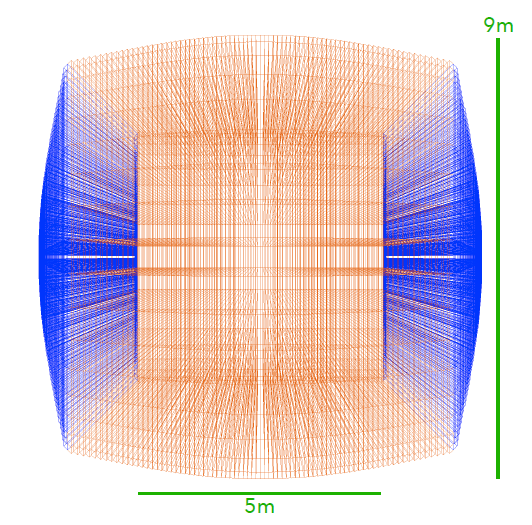
\includegraphics[width=0.6\textwidth]{IMG/DRCGeometry3}
%	\caption{Calorimeter geometry.}
%	\label{fig:cal_geometry}
%\end{figure}
\begin{figure}
	\centering
	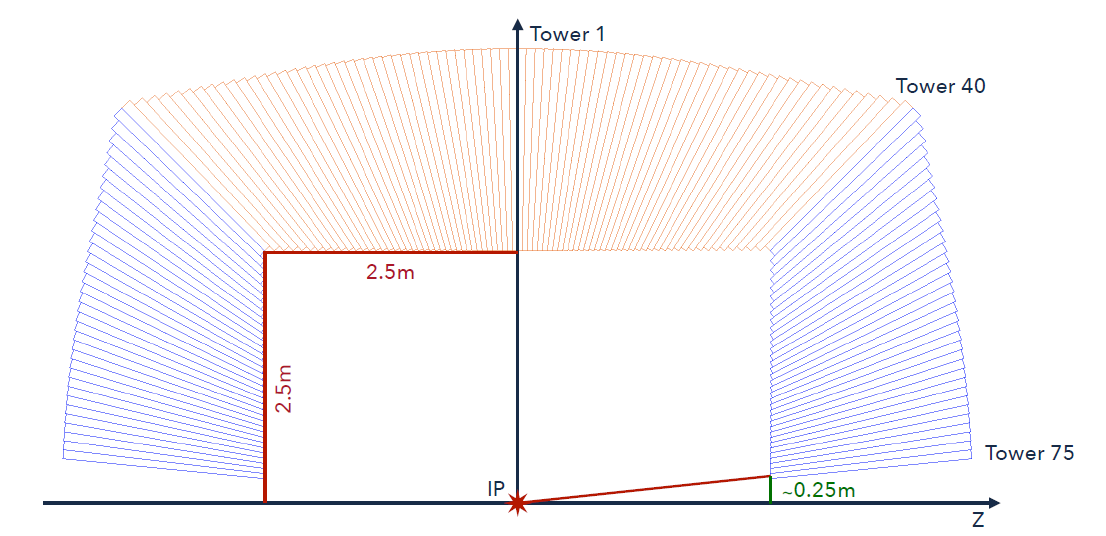
\includegraphics[width=0.8\textwidth]{IMG/DRCGeometry1}
	\caption{A calorimeter slice.}
	\label{fig:cal_slices}
\end{figure}

At present, the towers are based on copper (or brass) matrices that play the role of absorber. To have a sensitive element they have longitudinally running holes where optical fibres are inserted. The need of a projective geometry makes the detector dimensions increasing with the distance from the IP. New holes (with new fibres) open up at different depths inside the calorimeter, whenever possible, to keep constant the sampling fraction.\\
As the dual-readout technique needs independent scintillating ($S$) and Cherenkov ($C$) signals, two types of fibres are used (fig. \ref{fig:CS_fibres}). Their characteristics are shown in tab. \ref{tab:fibres}.\\
The fibre refractive indices determine the light transport (as consequence of the Snell's law). The signal from the scintillating fibres is parametrised by the deposited energy while the Cherenkov photons are produced accordingly to the Cherenkov emission process.\\

\begin{table}
	\centering
	\setlength{\tabcolsep}{12pt}
	\begin{tabular}{lp{0.6\textwidth}}
		\toprule
		\multicolumn{2}{c}{\textbf{Kuraray SCSF-78 ($S$)}}	\\
		\midrule
		Core:				& $r = 0.485\ mm$, Polystyrene ($C_5H_5$), $\rho=1.95\ g/cm^3$, $n = 1.59$	\\
		Cladding: 			& Thickness $=2\%$ of $r$, PMMA ($C_5H_8o_2$), $\rho=1.19\ g/cm^3$, $n=1.49$	\\
		Main properties:	& Emission constant $= 2.8\ ns$, LY $= 10^4\ \text{photons}/MeV$, $\lambda_{att} = 4\ m$	\\
		\midrule
		\multicolumn{2}{c}{\textbf{Mitsubishi SK-40 ($C$)}}	\\
		\midrule
		Core:				& $r = 0.485\ mm$, PMMA ($C_5H_8o_2$), $\rho=1.19\ g/cm^3$, $n = 1.49$	\\
		Cladding: 			& Thickness $=2\%$ of $r$, Fluorinated Polymer ($C_2F_2$), $\rho=1.43\ g/cm^3$, $n=1.42$	\\
		Main properties:	& $\lambda_{att} = 8.9\ m$	\\
		\bottomrule
	\end{tabular}
	\caption{Technical characteristics of the two type of fibres used.}
	\label{tab:fibres}
\end{table}

\begin{figure}
	\centering
	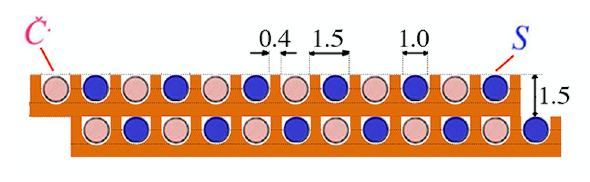
\includegraphics[width=0.8\textwidth]{IMG/DRCGeometry2}
	\caption{Chess-like configuration to dispose the fibres in the copper structure.}
	\label{fig:CS_fibres}
\end{figure}

For each event, the simulation produces as output the following information: 
\begin{itemize}
	\item Event ID;
	\item Fibre Type;
	\item Fibre ID;
	\item the position of the fibre end closer to the IP;
	\item the number of photons reaching the fibre further end;
	\item the list of photon times of arrival to the fibre end.
\end{itemize}

The computation of the light propagation is extremely time consuming, so that it has to be fine tuned to optimize the process. In particular, the propagation of $C$ photons is tracked until the single photon reach the core-cladding boundary (i.e. at the distance $R$ from the further end of the fibre and at the time $t_0$). If the emission angle is inside the range of the fibre numerical aperture, the photon is added to the final number of photons (after a Poissonian smearing on their number).
The time of arrival on the sensor for each photon is estimated as:
\begin{equation}
t_C = t_0 + R \frac{n_C}{c}
\end{equation}
where $n_C = 1.49$ is the fibre refractive index and $c$ is the speed of light.\\

The $S$ fibres, instead, carry scintillating photons produced considering the light yield of the fibres and the energy deposited by the interacting particle. The number of photons is smeared with a Poissonian law and the time of arrival on the sensor is obtained as:
\begin{equation}
	t_S = t_0 + R\frac{n_S}{c\cdot \cos(\vartheta)} + t^*
\end{equation}
where $n_S = 1.59$ is the refractive index and $t^*$ is a random time that accounts for the scintillator decay time, chosen from an exponential distribution with $2.8\ ns$ as mean value.
Considering the internal reflection, the photon path depends on the $\vartheta$ angle (i.e. the angle between the photon direction and the fibre axis). It is chosen randomly in the range $[\cos(\alpha),\cos(0)]$, where $\alpha = 20.4\degree$ is the fibre critical angle.\\
Eventually, the light produced is smeared by two Poissonian distribution, one for the scintillation signal and the other for the Cherenkov one. This procedure correctly reproduces the statistical fluctuations in the scintillation and Cherenkov light production and allows to reproduce within the simulations the desired light yields (p.e./GeV). To make the full simulation lighter, this process also includes the attenuation due to the PDE of the simulated SiPMs. The simulation is tuned to produce $\sim 400\ Spe/GeV$ and $\sim 100\ Cpe/GeV$ at the electromagnetic scale.

\subsection{SiPM response digitization} \label{subsec:Sim_SiPM}
The results obtained are the input of the second part of the simulation: \textit{pySiPM}, a Monte Carlo simulation, performed mostly in Python, able to reproduce the SiPM response to a light source and replicate the waveforms recorded with a digitizer \cite{digitizer}.\\

The importance of this software goes beyond our context, but perfectly fits our needs. In particular each fibre from the calorimeter simulation is considered coupled to a single SiPM, which digitized response is simulated through \textit{pySiPM}.

The simulation allows to set most of the SiPM parameters:
\begin{itemize}
	\item \textbf{Geometrical parameters}: the sensor dimensions and the pixel pitch.
	\item \textbf{Sensor parameters}: Photon Detection Efficiency, Dark Count Rate, After-Pulse probability, Optical Cross-Talk probability.
	\item \textbf{Signal parameters}: rise time constant, decay time constant.
	\item \textbf{Waveform parameters}: time window, sampling time, integration window.
\end{itemize}

For each event and fibre, random parameters determine the photon position inside the sensor. %Meanwhile the sensor PDE is tuned to have consistent mean values of $\sim 400\ Spe/GeV$ and $\sim 100\ Cpe/GeV$ respectively for $S$ and $C$ light yield.
Meanwhile the sensor PDE is set at $100\%$ to be consistent with the smearing applied at the calorimeter simulation level.
A control stops the count of impinging photons on the same cell to a maximum of one, then each element of noise is generated with the set probability.\\
The generated pulse is a combination of two exponentials characterized by the rise time constant ($\tau_{rise}$) and the decay time constant ($\tau_{fall}$), considering the different photon time of arrival ($t_S$ and $t_C$):
\begin{equation}
	y(t)= A \cdot \left( e^{-\frac{t}{\tau_{fall}}} - e^{-\frac{t}{\tau_{rise}}}\right).
	\label{form:resp_func}
\end{equation}

The output signal for any given SiPM is the sum of all the signals generated by the activated cells.\\

The information given as output of the simulation are:
\begin{itemize}
	\item \textbf{Data reported from GEANT4 simulation}: event ID, type of fibre, fibre ID, fibre position;
	\item \textbf{Computated quantities}: integral, peak height, time of arrival, time over threshold, time of peak;
	\item \textbf{Digitized waveform}.
\end{itemize}

All this features can be rejected through a trigger, in particular a threshold can be set to establish the information that has to be recorded.
The threshold is defined as a scale factor of the maximum value of the waveform generated by a single photoelectron (neglecting the electrical noise). In the results shown later a one-suppression has been applied using a threshold factor of $1.5$, a typical setup to filter isolated signals due to the DCR.\\

\section{Simulation performances} \label{sec:Sim_perf}

\subsection{Different configurations} \label{subsec:SiPM_conf}
The results shown in this chapter are obtained considering different SiPM parameter configurations.\\
They have been chosen in a common parameter space identified by checking the lineup of SiPMs produced by Hamamatsu \cite{SiPM_lineup}. 
Two are the parameters that has been changed in our studies: 
\begin{itemize}
	\item the decay time constant of the signal, the chosen values being $10\ ns$ and $50\ ns$;
	\item the pixel size, the chosen values being $10\ \mu m$, $15\ \mu m$ and $25\ \mu m$.
\end{itemize}

The other parameters have not been modified for this work. Their values are listed in the table \ref{tab:SiPM_par}.\\

\begin{table}
	\centering
	\setlength{\tabcolsep}{18pt}
	\begin{tabular}{ll}
		\toprule
		\multicolumn{2}{c}{\textbf{Geometrical Parameter}}	\\
		SiPM area	& $1 \times 1\ mm^2$	\\
		\midrule
		\multicolumn{2}{c}{\textbf{Sensor Parameters}}	\\
		DCR			& $200 \ kHz$	\\
		After-Pulse	& $3\% $	\\
		Cross-Talk	& $1\% $	\\
		\midrule
		\multicolumn{2}{c}{\textbf{Signal Parameter}}	\\
		Rise time	& $1\ ns$	\\
		\midrule
		\multicolumn{2}{c}{\textbf{Waveform Parameters}}	\\
		Time window	& $500 \ ns$	\\
		Integration window	& $300 \ ns$	\\
		Sampling frequency	& $10\ GHz$	\\
		\bottomrule
	\end{tabular}
	\caption{Fixed SiPM parameters used in the simulation configuration file. For the values of the variable parameters see the text.}
	\label{tab:SiPM_par}
\end{table}

An example of generated waveform is plotted in figure \ref{fig:diff_wf} where it is clear the impact of the two different decay-time constants.

\begin{figure}
	\centering
	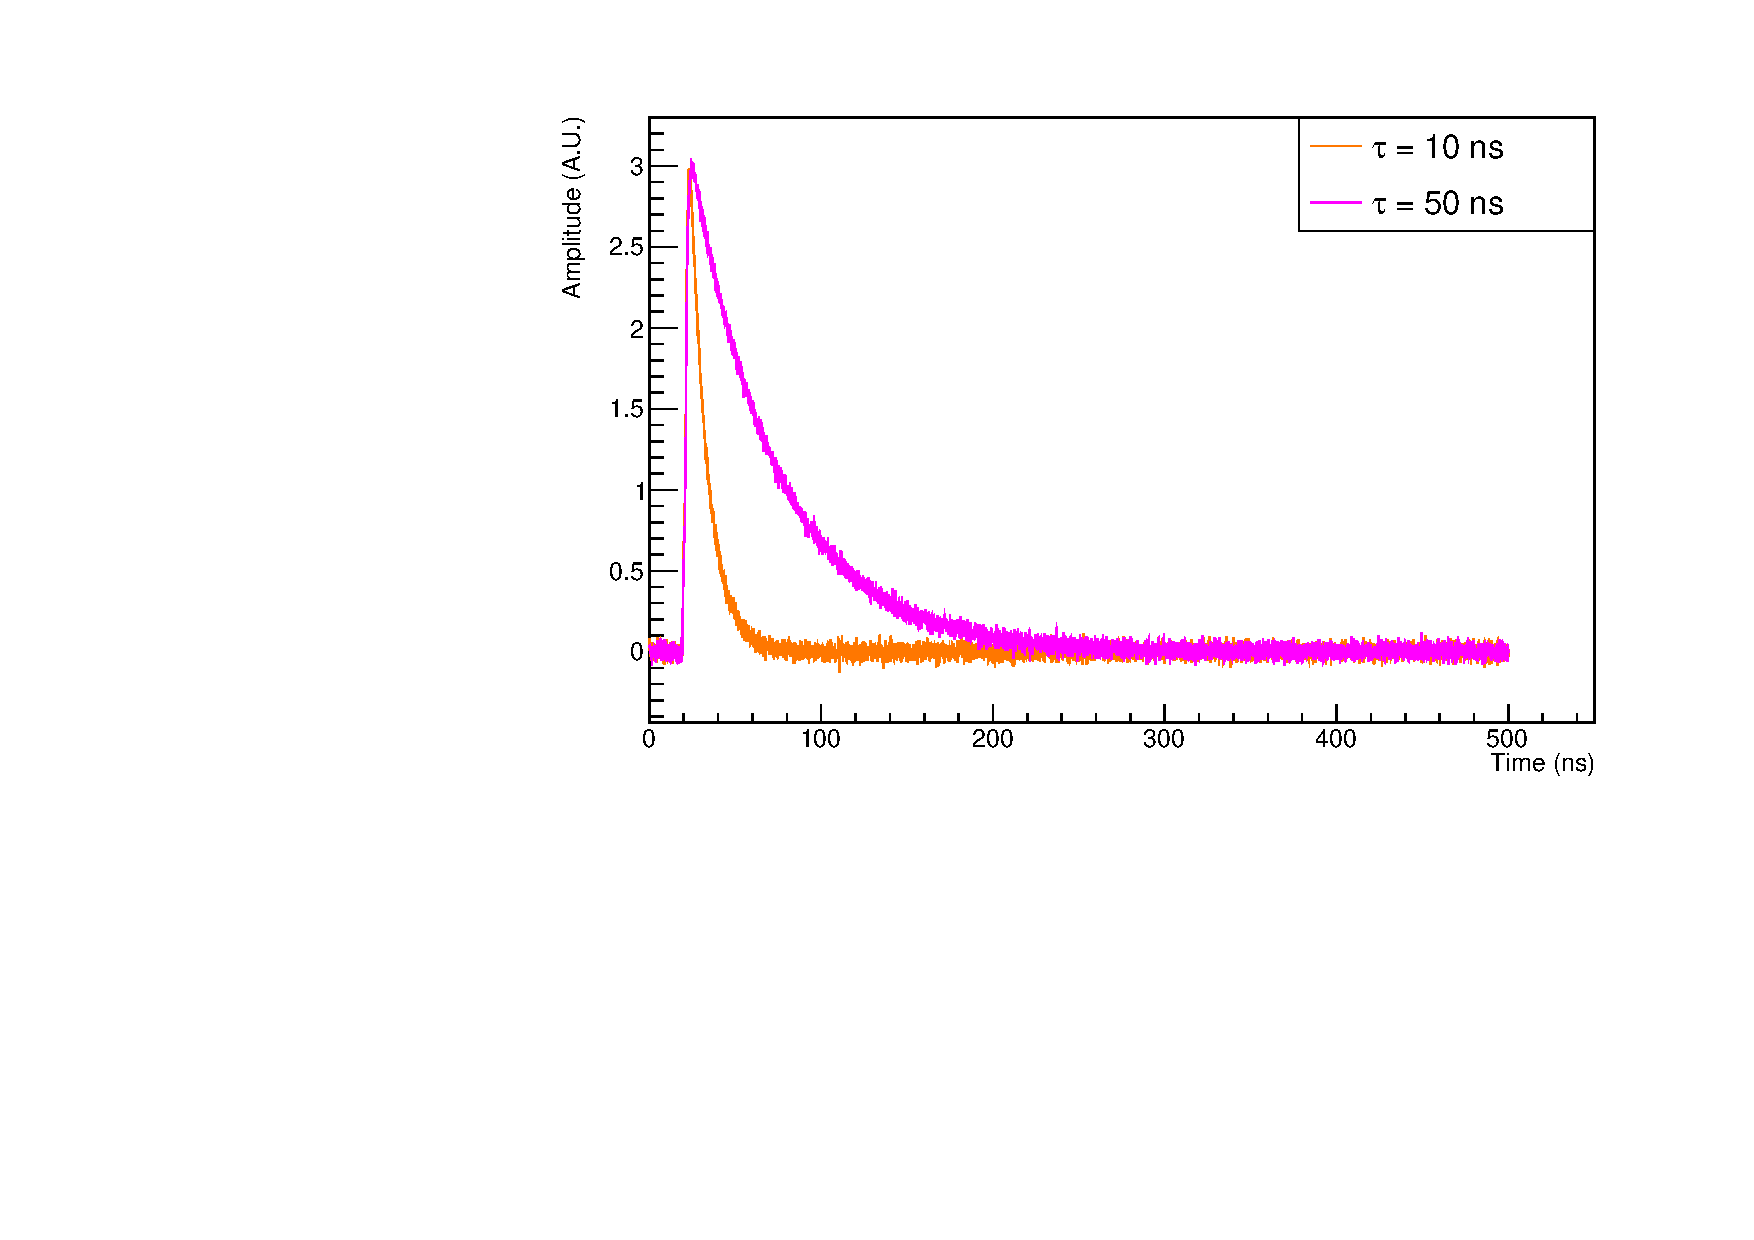
\includegraphics[width=0.8\textwidth]{IMG/Cap5/wf_different_conf}
	\caption{Single waveforms generated in two identical conditions except for the decay-time constant.}
	\label{fig:diff_wf}
\end{figure}

\subsection{Time studies} \label{subsec:Time}
An important aspect that has to be studied is the temporal evolution of the signals.
For that, data of $1000$ events have been generated. In each event a $20\ GeV$ electron is produced at the interaction point.\\
A first step is to analyze the distribution of the time of arrival of the photons converted at the SiPMs (i.e. the time recorded in the GEANT4 simulation output).\\
The distributions obtained from $C$ and $S$ photons are plotted in figure \ref{fig:true_toa_dist}.
As expected, the distribution of $C$ photons time extremely narrow due to the instantaneous production of photons at the passage of relativistic charged particle in the fibres, instead the $S$ photons time distribution shows an exponential tail that is a direct consequence of the emission time constant of the Polystyrene ($\tau = 2.8\ ns$).\\

\begin{figure}
	\centering
	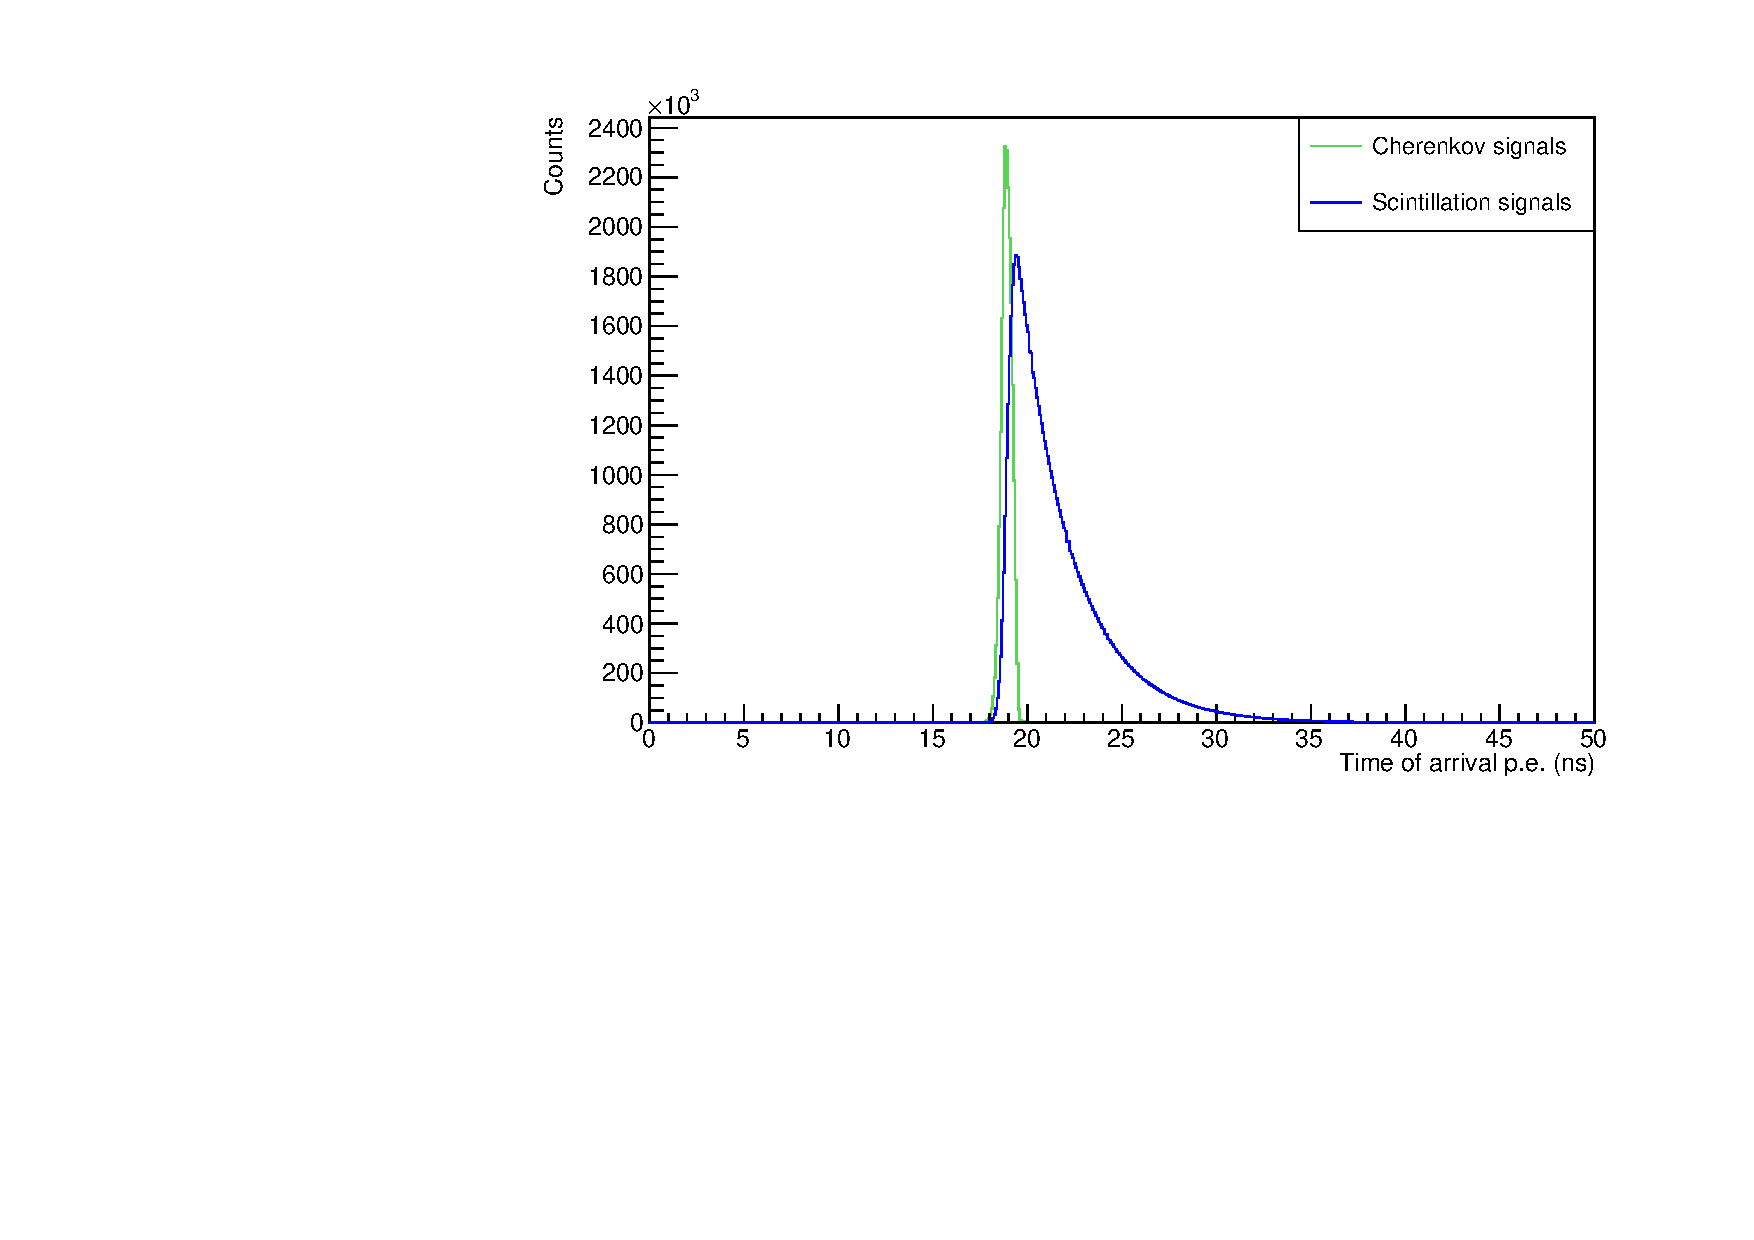
\includegraphics[width=0.8\textwidth]{IMG/Cap5/TrueTimeDist20GeV}
	\caption{The distributions of the time of arrivals of photons on the SiPMs surface, distinguishing the ones transported from Cherenkov fibres from the ones transported from scintillation fibres.}
	\label{fig:true_toa_dist}
\end{figure}

Now a step forward can be done using this data as input for \textit{pySiPM}. The SiPM parameters are chosen as described in paragraph \ref{subsec:SiPM_conf}. In this context the most interesting editable parameter is the decay time constant.\\ 
Figure \ref{fig:top_50ns} and \ref{fig:top_10ns} are in analogy with respect to the last described and presents clearly a widening of the distributions, the cause of this phenomenon has to be associated to the characteristic response function of the sensors \ref{form:resp_func}.\\
These data can be compared looking for differences in changing SiPMs configurations. As we can see in figure \ref{fig:top_per_fib}, the same $C$ and $S$ photons produce narrower time of peak distribution due to the less impact of electronic noise on a sharper response function.\\

\begin{figure}
	\centering
	\subfloat[][\label{fig:top_10ns}$\tau_{fall} = 10\ ns$.]{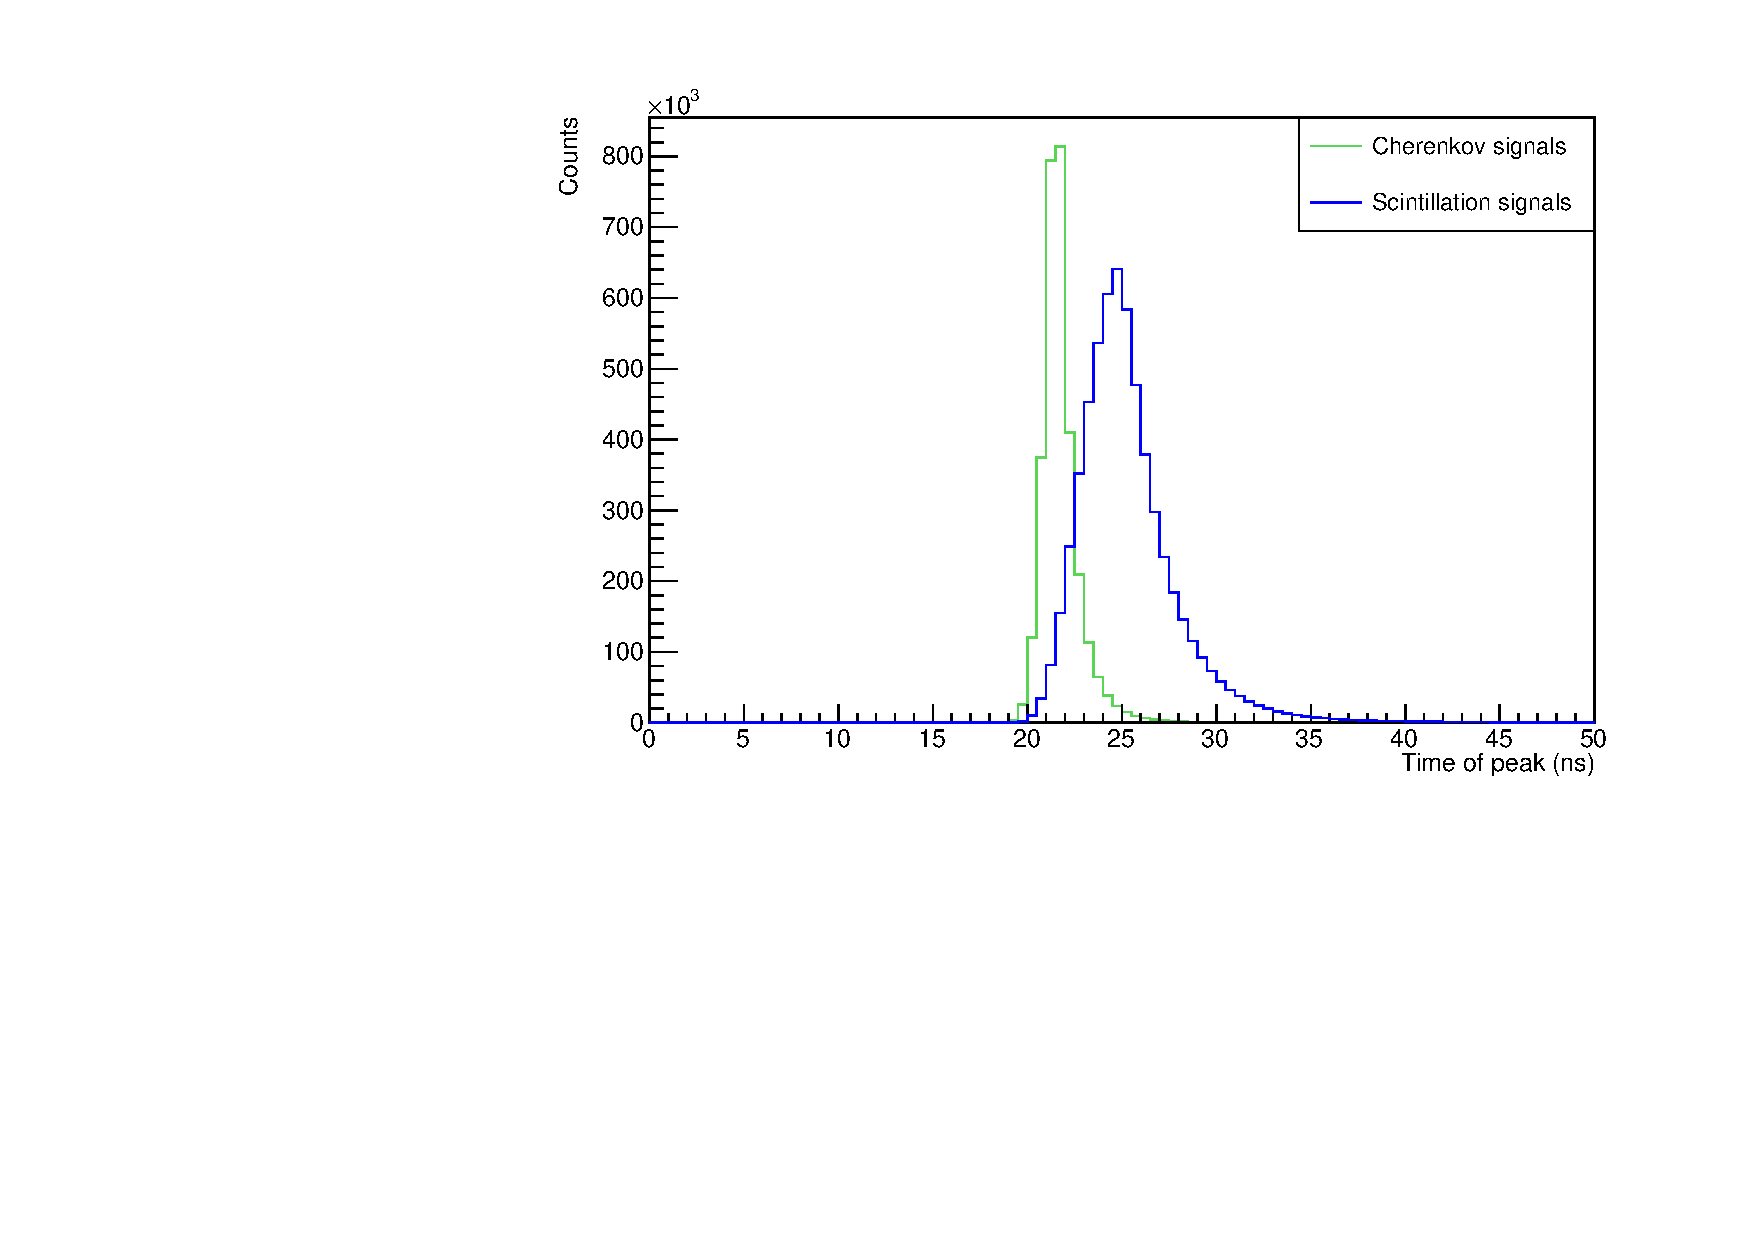
\includegraphics[width=.45\textwidth]{IMG/Cap5/ToP_20GeV_10ns}} \quad
	\subfloat[][\label{fig:top_50ns}$\tau_{fall} = 50\ ns$.]{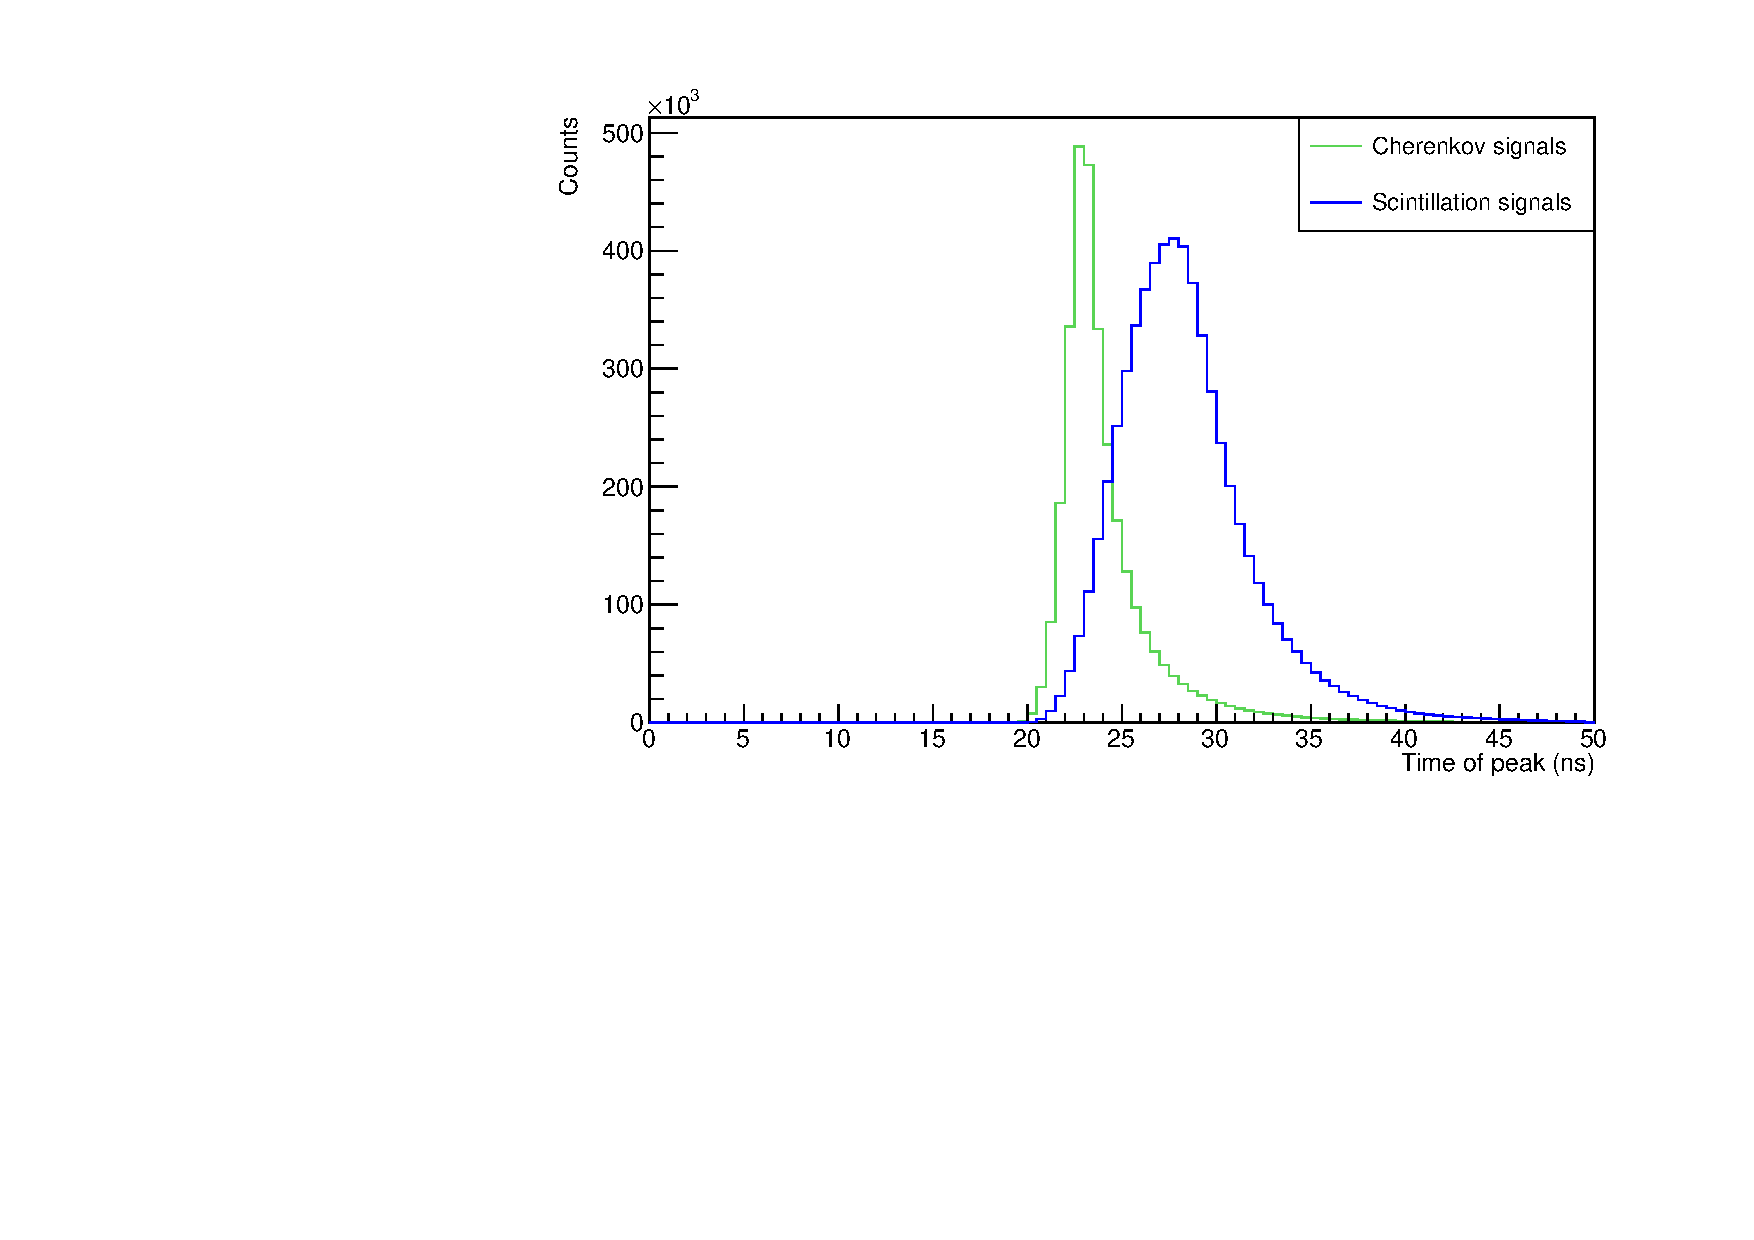
\includegraphics[width=.45\textwidth]{IMG/Cap5/ToP_20GeV_50ns}}
	\caption{Time of peak distributions comparing in each histogram signals from Chernkov and from scintillation fibres. Different figures correspond to different decay time constants.}
	\label{fig:top_per_tau}
\end{figure}

\begin{figure}
	\centering
	\subfloat[][\label{fig:top_C}Cherenkov fibres.]{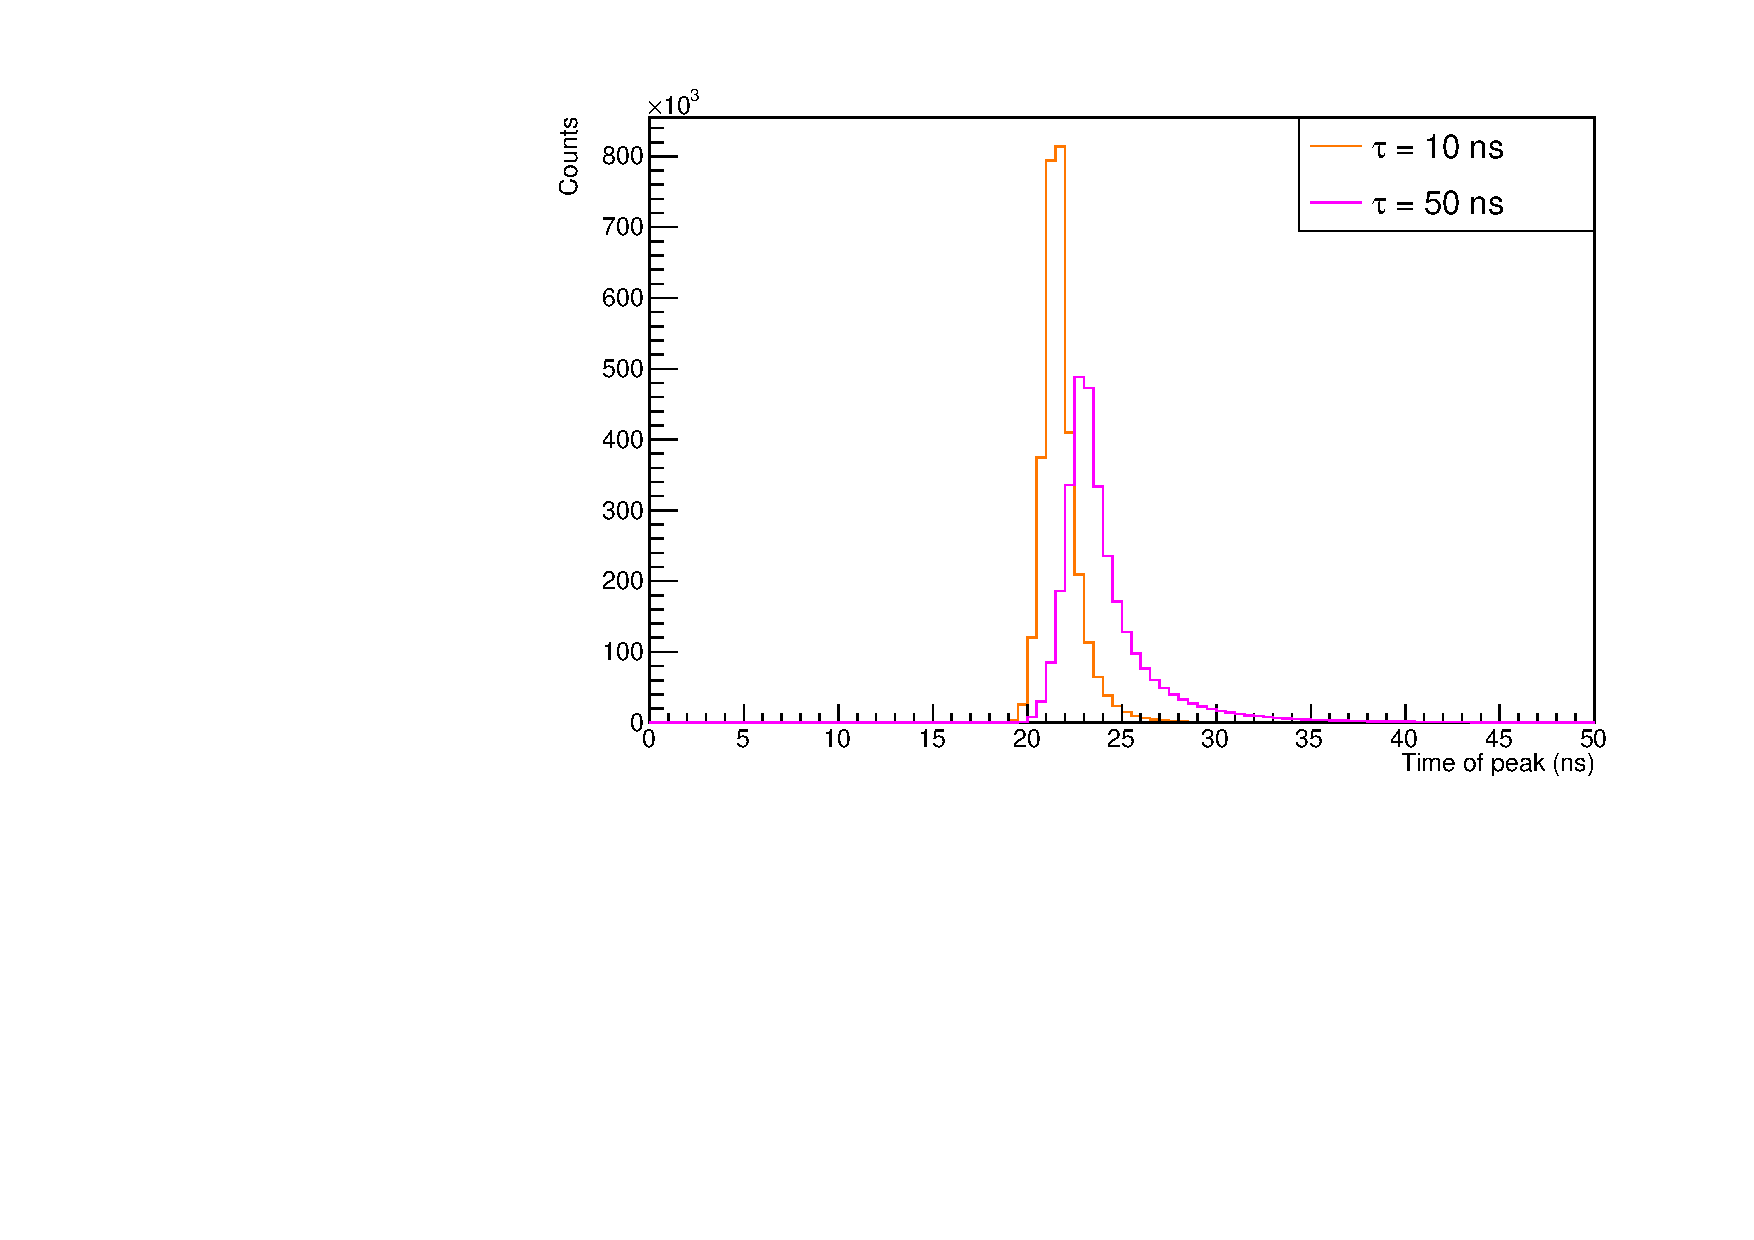
\includegraphics[width=.45\textwidth]{IMG/Cap5/ToP_20GeV_cher}} \quad
	\subfloat[][\label{fig:top_S}Scintillation fibres.]{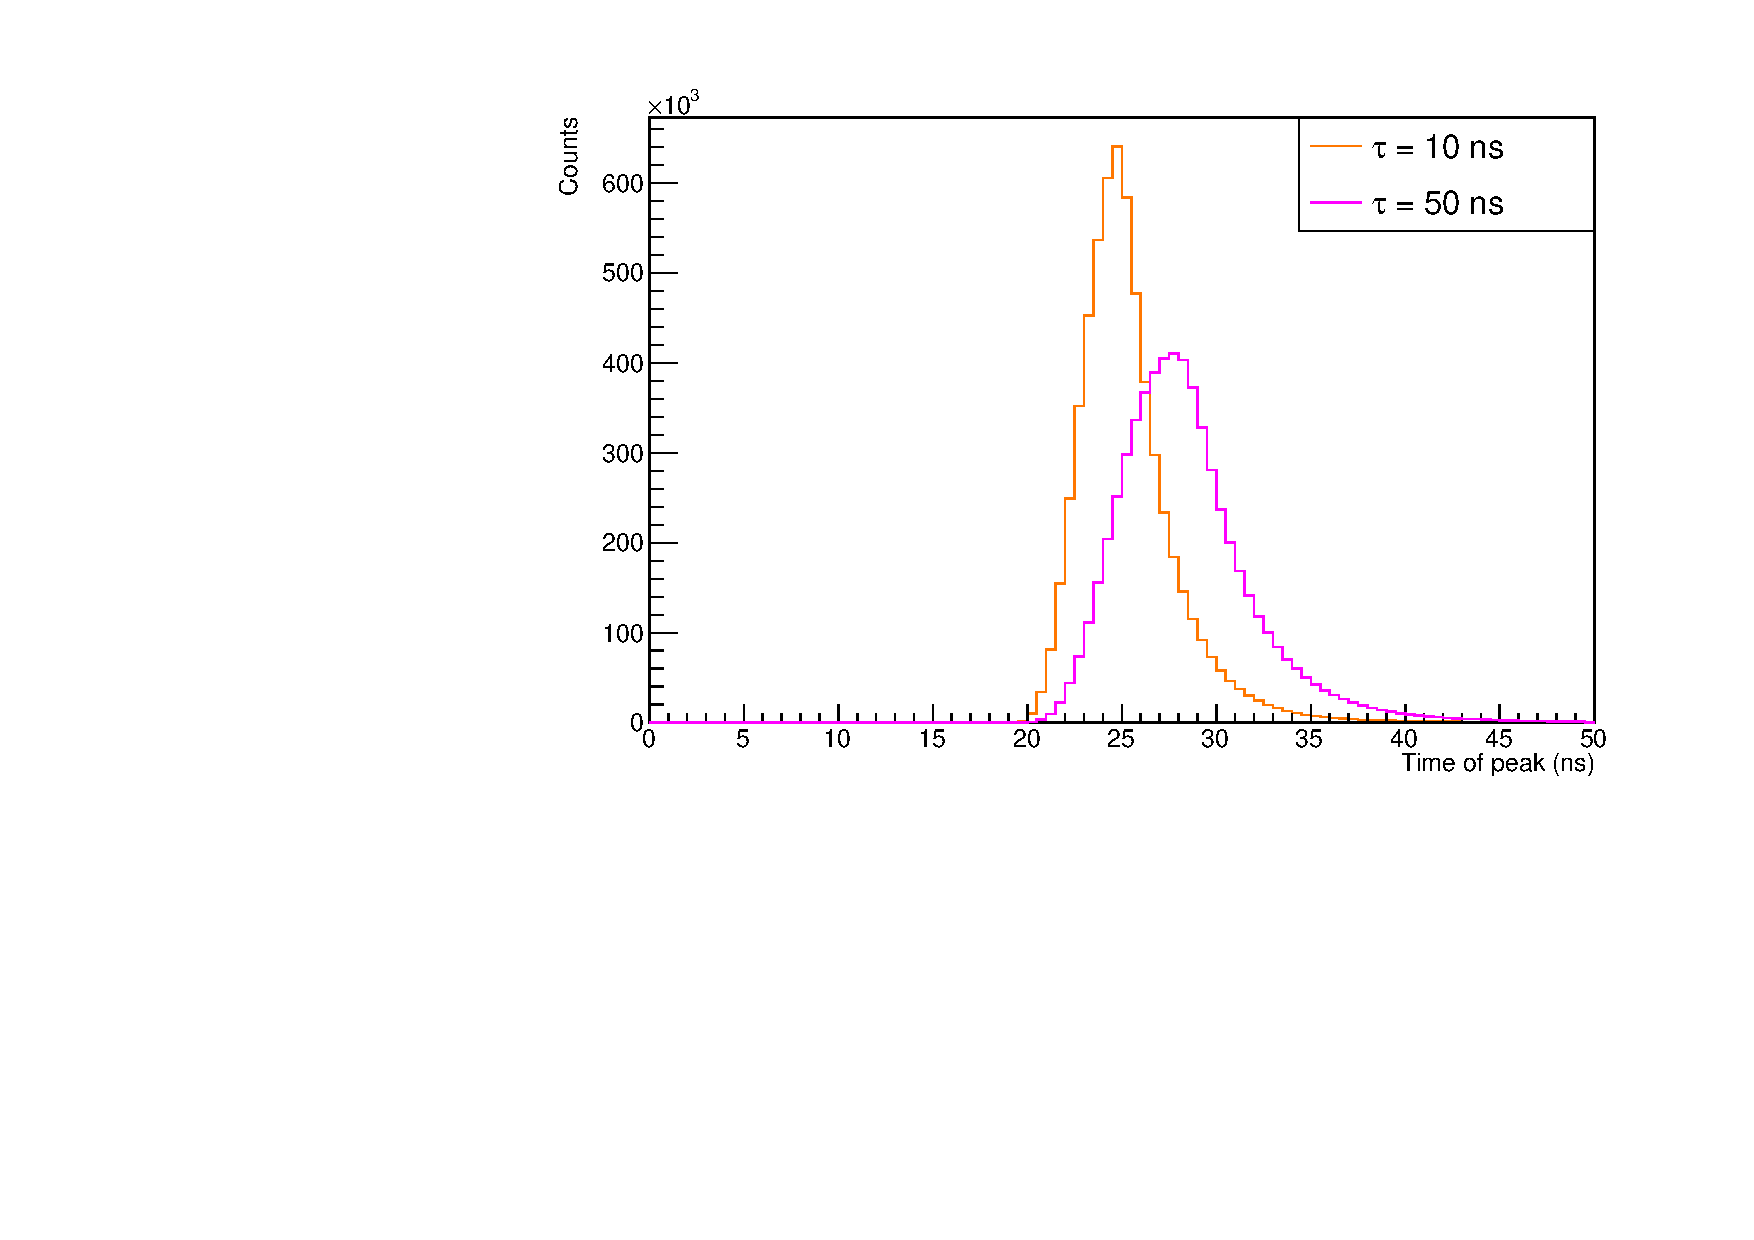
\includegraphics[width=.45\textwidth]{IMG/Cap5/ToP_20GeV_scin}}
	\caption{Time of peak distributions comparing in each histogram signals with different decay time constant of SiPMs. Different figures correspond to different photon emission processes.}
	\label{fig:top_per_fib}
\end{figure}

The impact of noise on time of peak precision is also dependent on the number of photons impinging the same SiPM, in particular the peak precision increase with the number of photons.\\
To prove this $10000$ SiPMs have been fired with an increasing number of simultaneous photons. For each fixed number of photons, the time of peak has been recorded, plotted in an histogram and fitted with a Gaussian function. An example of these histograms is shown in figure \ref{fig:top_dummy}.\\

The standard deviation of these Gaussian fit is the interested quantity that has been recorded and reported in the table \ref{tab:sigmas}.\\
It is interesting to plot these data and study the behavior of the standard deviation in fuction of the number of photons. Figure \ref{fig:top_sigma} shows graphically the data, which are well fitted with a function of the form:
\begin{equation}
	\sigma = \frac{A}{\sqrt{n}} + B.
\end{equation}
The parameters obtained are $A = 0.8712\ ns$ and $B = 0.08734\ ns$ for data associated to SiPMs with $\tau_{fall}=10\ ns$, and $A = 1.949\ ns$ and $B = 0.008217\ ns$ for data associated to SiPMs with $\tau_{fall}=50\ ns$.

\begin{table}
	\centering
	\begin{tabular}{lcc}
		\toprule
		Number of photons	& $\sigma$ with $\tau_{fall}=10\ ns$ (ns) & $\sigma$ with $\tau_{fall}=50\ ns$ (ns)	\\
		\midrule
		$1$ 	& $1.4150$ & $7.0680$ \\
		$2$ 	& $0.8717$ & $2.6420$ \\
		$3$ 	& $0.6738$ & $1.7370$ \\
		$4$ 	& $0.5742$ & $1.3770$ \\
		$5$ 	& $0.5146$ & $1.1230$ \\
		$6$ 	& $0.4624$ & $0.9719$ \\
		$7$ 	& $0.4314$ & $0.9148$ \\
		$8$ 	& $0.3998$ & $0.8508$ \\
		$9$ 	& $0.3811$ & $0.7717$ \\
		$10$ 	& $0.3605$ & $0.7169$ \\
		$25$ 	& $0.2339$ & $0.4481$ \\
		$50$ 	& $0.1679$ & $0.3112$ \\
		$100$ 	& $0.1229$ & $0.2297$ \\
		\bottomrule
	\end{tabular}
	\caption{Standard deviations obtained through the Gaussian fit applied on the time of peak distributions under different conditions. }
	\label{tab:sigmas}
\end{table}

\begin{figure}
	\centering
	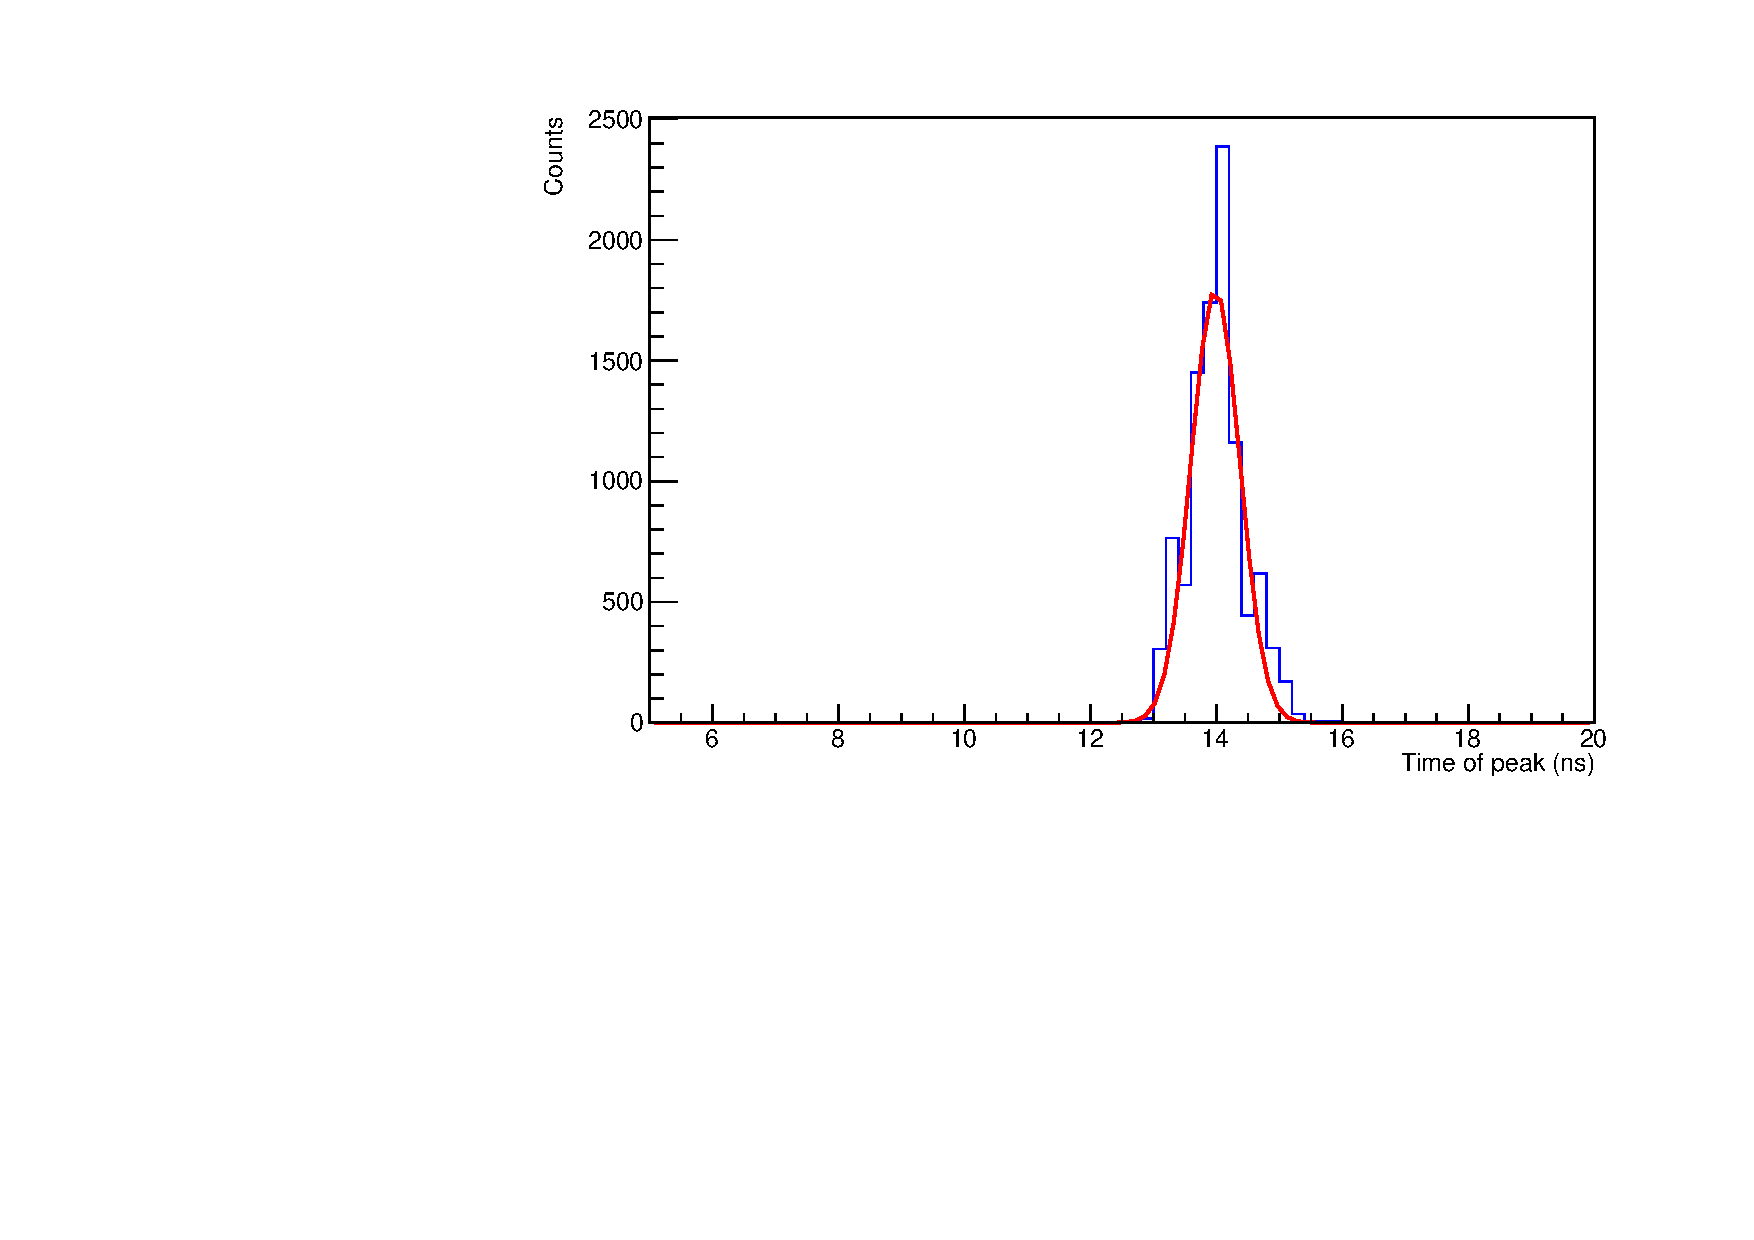
\includegraphics[width=0.8\textwidth]{IMG/Cap5/Dummy11pe_50ns}
	\caption{Time of peak distribution obtained firing $10000$ SiPMs with $11$ photoelectrons each, all at the same time ($10 ns$). Over this distribution a Gaussian fit has been applied.}
	\label{fig:top_dummy}
\end{figure}

\begin{figure}
	\centering
	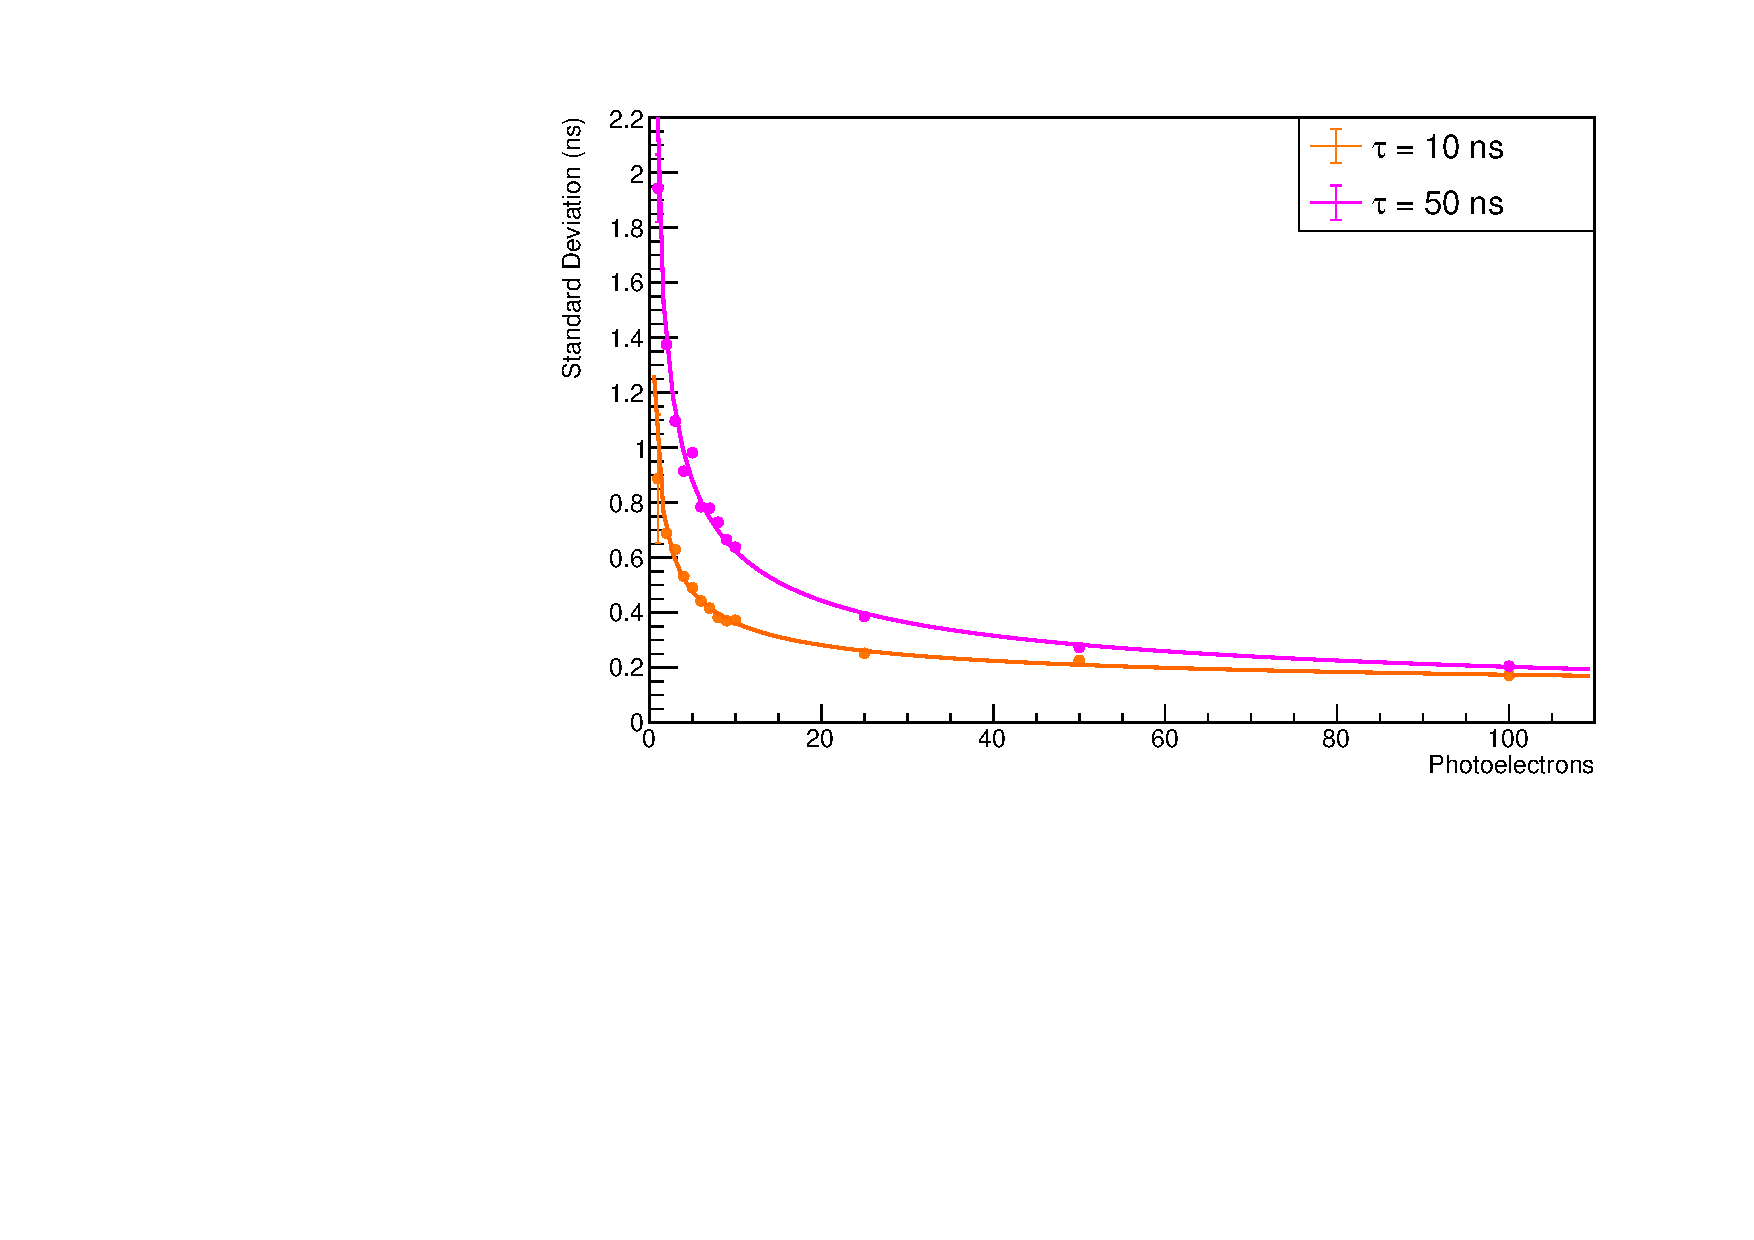
\includegraphics[width=0.8\textwidth]{IMG/Cap5/PeakSpread}
	\caption{Standard deviation behaviour with respect to the number of simultaneous photoelectrons. Study performed with two different decay time constant in SiPMs configuration.}
	\label{fig:top_sigma}
\end{figure}


\subsection{Occupancy effect} \label{subsec:Sat_effect}
The occupancy effect, as shown in the paragraph \ref{sec:SiPM_work}, is an important characteristic that has to be deeply studied to know the behaviour of the SiPMs under high number of impinging photons and to correctly reconstruct the released energy.\\

As can be seen in figure \ref{fig:sat_example}, this effect is reproduced correctly in our simulations. The example shows the charge integral in dependence to the number of p.e. and follows the concepts already seen in paragraph \ref{subsec:occupancy_teo}.\\

\begin{figure}
	\centering
	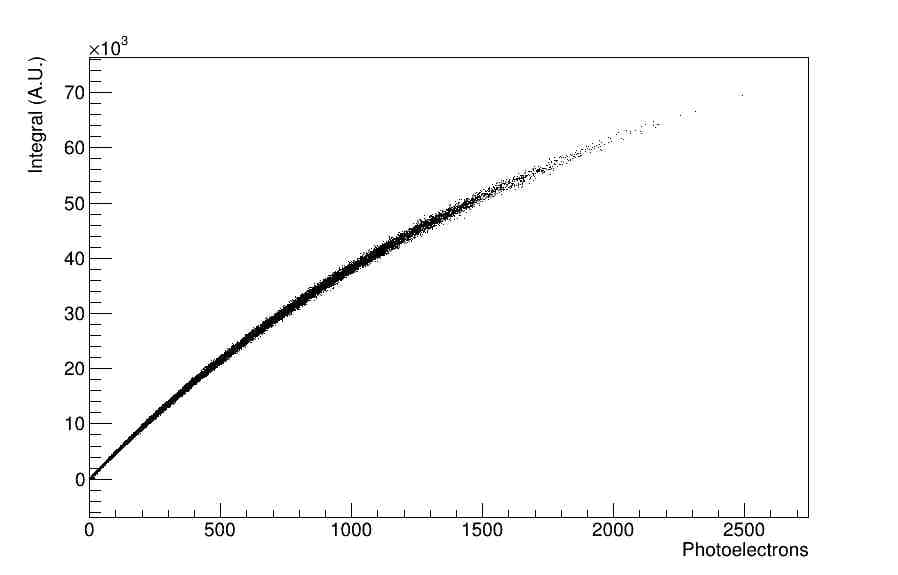
\includegraphics[width=0.7\textwidth]{IMG/Cap5/SatExample.jpg}
	\caption{Example of saturation effect produced with the simulation chain. Each point correspond to a SiPM with a cell size of $25\ \mu m$.}
	\label{fig:sat_example}
\end{figure}

The first step to perform these studies is to reconstruct a calibration law that reproduces the charge integral with respect to the number of p.e. firing the same SiPM.\\
Starting by assuming that in the range of photoelectrons from $2$ to $10$ the saturation effect does not occur in our configurations (i.e. $10000$, $4356$ and $1600$ cells in each SiPM), $10000$ SiPM has been fired $9$ times with an increasing number of simultaneous p.e. in the range considered.\\
To assume that no saturation effect occurs in these data the charge integral distribution from the three different configurations has been compared finding no bias as seen in figure \ref{fig:SatCheck}. The mean and the RMS values has been recorded and fitted with a strait line corresponding to the calibration law desired:
\begin{equation}
	I(n) = A \cdot n + B
\end{equation}
with $A = 49.43 \pm 0.03852$ and $B = 2.491 \pm 0.2516$ (fig \ref{fig:NoSatLine}).\\
The parameter $A$ represents the contribution to the charge integral associated to a single photoelectron. Meanwhile $B$ is the pedestal that is originated mostly by the DCR. This contribution can be evaluated considering our parameters of DCR $= 200\ kH$ and the integration window of $300\ ns$.
$B_{DCR} = 2 \cdot 10^5 \cdot 3 \cdot 10^{-7} p.e. = 6\cdot 10^{-2} p.e. = 6\cdot 10^{-2} \cdot 49.43 = 2.96$.\\
In the following result, the value of the pedestal has been subtracted to the integral value of each SiPM.\\

\begin{figure}
	\centering
	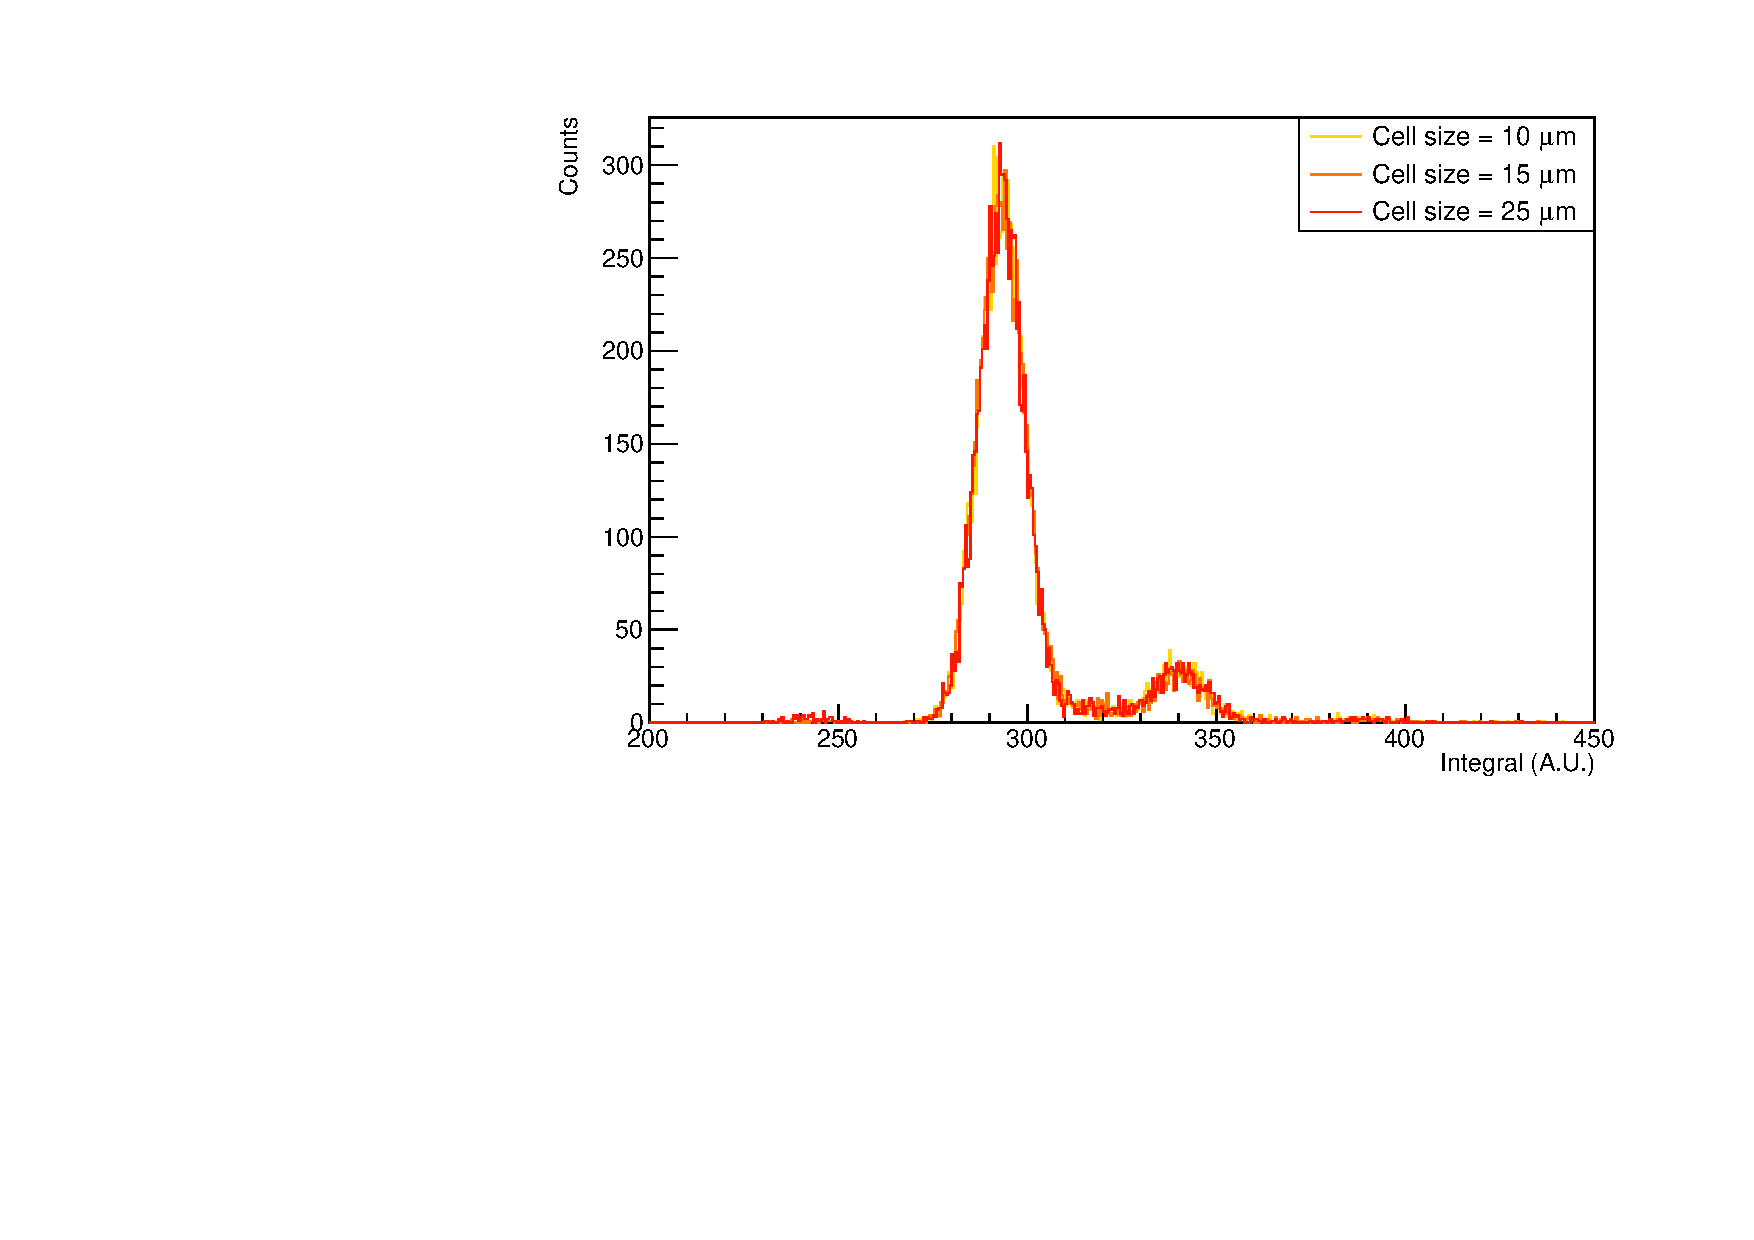
\includegraphics[width=0.7\textwidth]{IMG/Cap5/6pe_sat}
	\caption{Charge integral distributions with different SiPM cell size considering $6$ simultaneous photoelectrons. The distribution shape with less then $10$ simultaneous p.e. is not dependent to the number of cells.}
	\label{fig:SatCheck}
\end{figure}

\begin{figure}
	\centering
	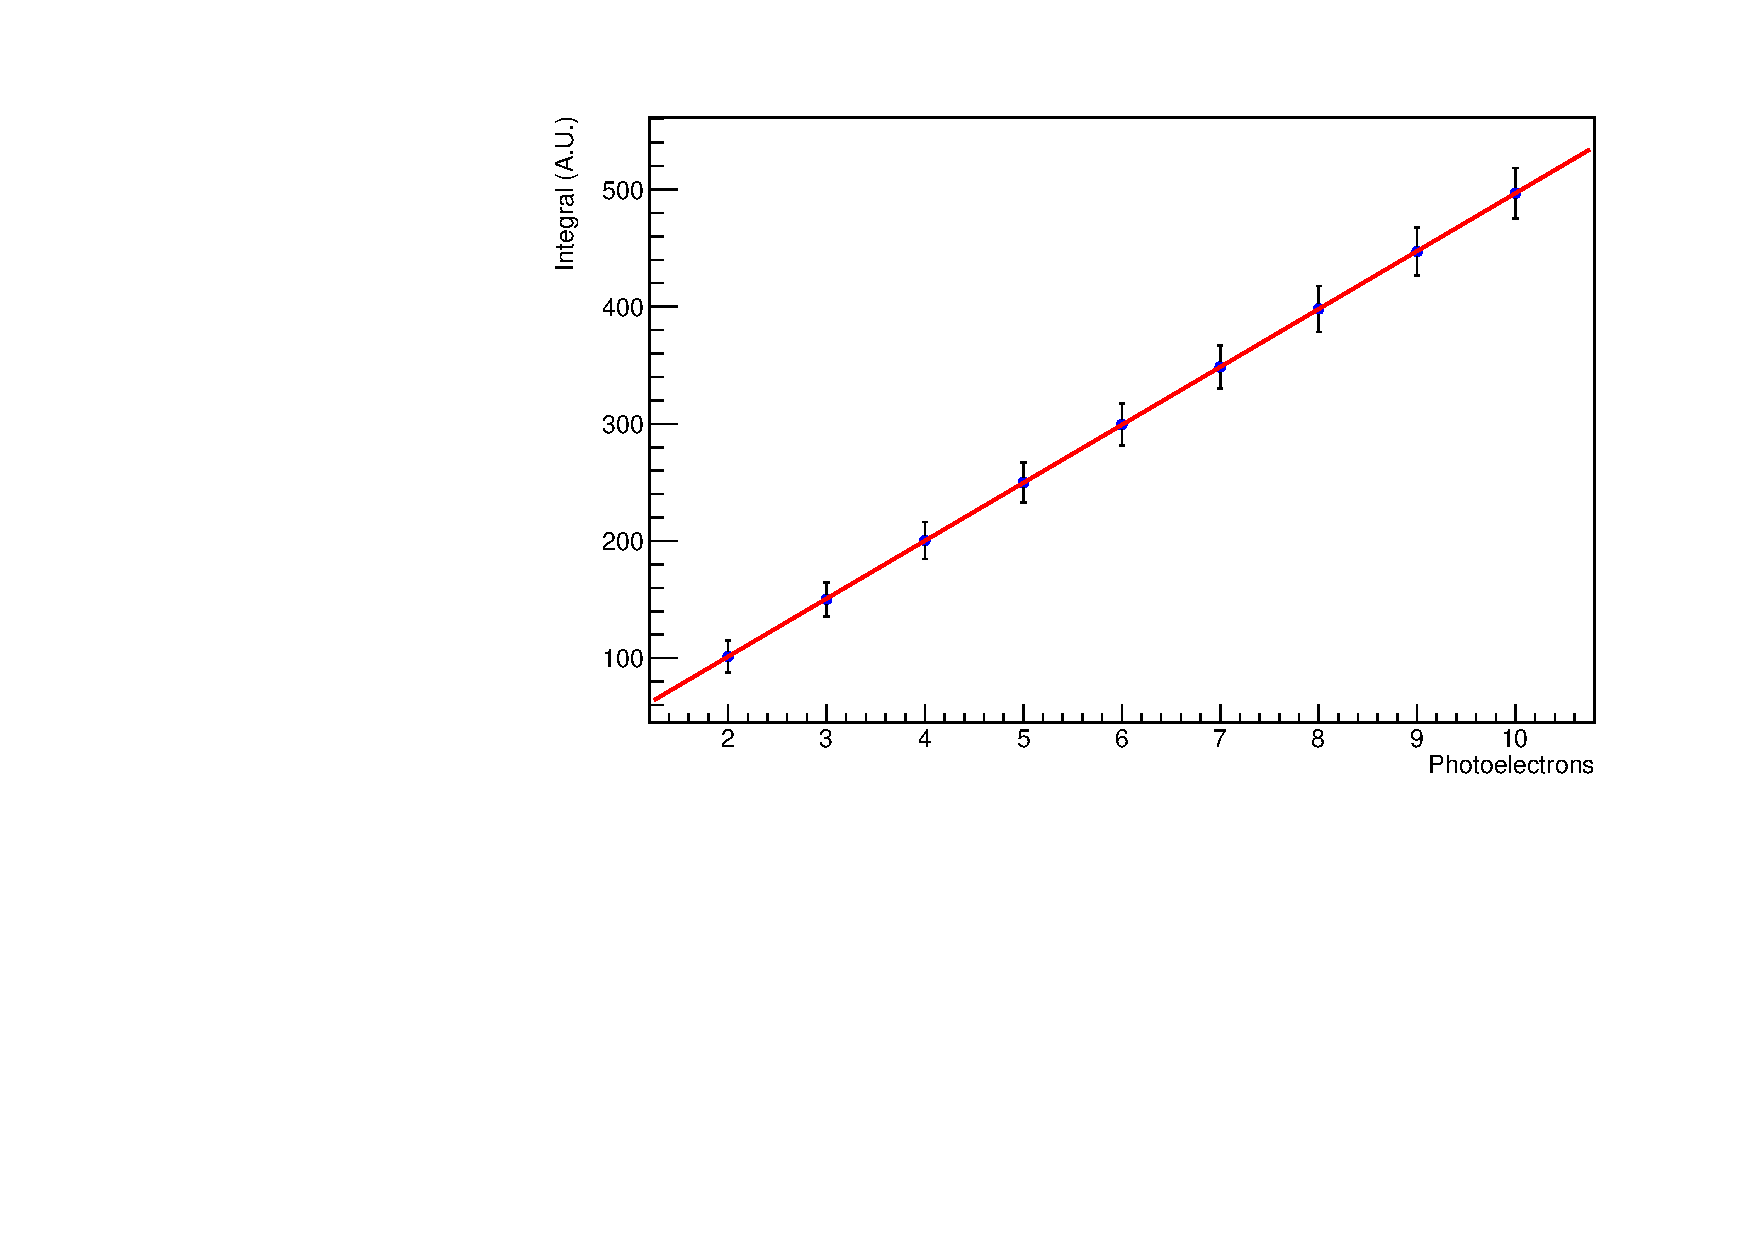
\includegraphics[width=0.7\textwidth]{IMG/Cap5/NoSatLine}
	\caption{Study of the proportional relation between integral and number of photoelectrons in the range from $2$ to $10$. A linear fit has been applied to find calibration law without saturation.}
	\label{fig:NoSatLine}
\end{figure}

The occupancy effect has been studied in electromagnetic shower produced by single electrons of different energies at each event with discrete values of $20,\ 40,\ 60,\ 80\ GeV$.\\
The impact of the saturation has been quantified using the line $I = A\cdot n$ as no saturation reference. The result obtained from $10000$ events of single $40\ GeV\ e^-$ with different SiPM configurations are separated in Cherenkov and Scintillation signals. They are shown in figure \ref{fig:sat_fibres} where each point correspond to a single SiPM. The smaller is the number of cells, the greater is the occupancy effect.\\
Moreover, as expected, the scintillation fibres transport $\sim 4$ times the p.e. from Cherenkov ones on average, therefore they are more affected to the saturation.\\

\begin{figure}
	\centering
	\subfloat[][Cherenkov signals.]{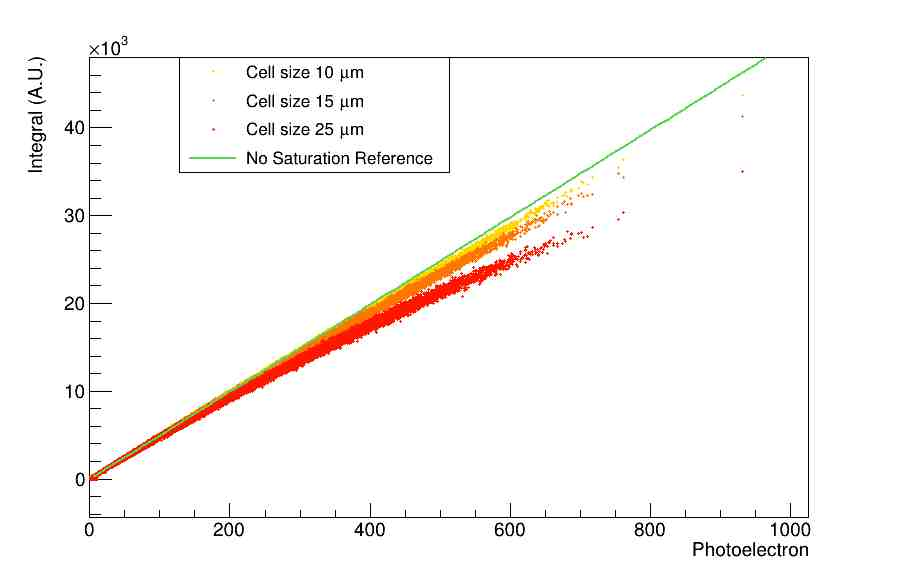
\includegraphics[width=.7\textwidth]{IMG/Sat_Fib_40GeV_cher}} \\
	\subfloat[][Scintillation signals.]{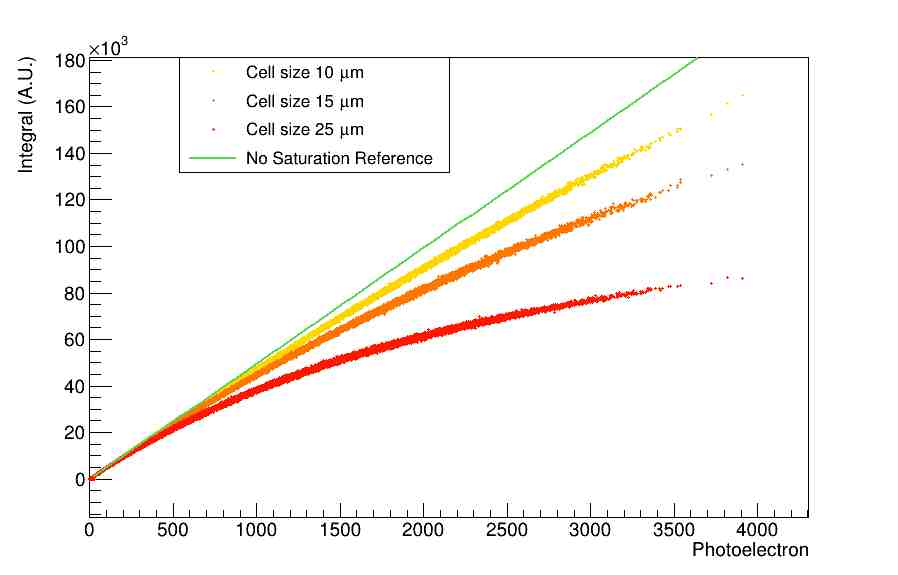
\includegraphics[width=.7\textwidth]{IMG/Sat_Fib_40GeV_scin}}
	\caption{The plots, divided considering the two different photon production processes, show the occurrence of the occupancy effect studying single $40\ GeV$ electrons. Each point correspond to a SiPM with different values of cell size. The no saturation line shown in figure \ref{fig:NoSatLine} has been added as reference.}
	\label{fig:sat_fibres}
\end{figure}

This process can be extended considering one event at the time and adding the charge integral and the corresponding number of photoelectrons. The effect produced is represented in figure \ref{fig:sat_events} where each point correspond to a single event.\\

\begin{figure}
	\centering
	\subfloat[][Cherenkov signals.]{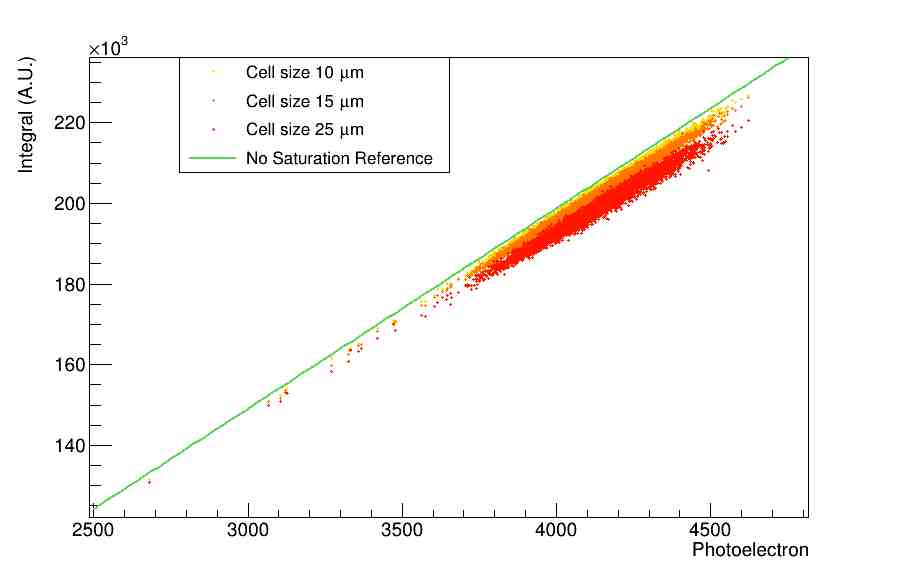
\includegraphics[width=.7\textwidth]{IMG/Sat_Ev_40GeV_cher}}\\
	\subfloat[][Scintillation signals.]{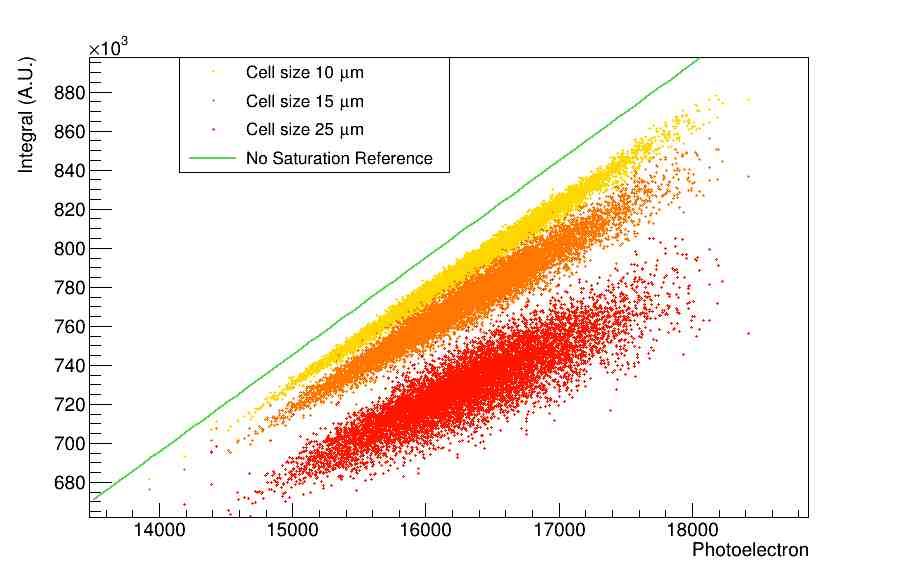
\includegraphics[width=.7\textwidth]{IMG/Sat_Ev_40GeV_scin}}
	\caption{The plots, divided considering the two different photon production processes, show the occurrence of the occupancy effect studying single $40\ GeV$ electrons. Each of the $10000$ points correspond to a single event where integral and number of photoelectrons have been added over the fired SiPMs. Different values of cell size are represented with different colors. The no saturation line shown in figure \ref{fig:NoSatLine} has been added as reference.}
	\label{fig:perc_sat}
\end{figure}

As can be seen, the occupancy effect in our conditions is consistent. To mitigate this problem an analytical correction can be performed through the formula:
\begin{equation}
	N_{fired}=N_{cells} \cdot \left[ 1 - \exp\left(-\frac{N_{p.e.}}{N_{cells}}\right)\right]
\end{equation}

therefore the correction has been applied modifying the integral values such as:
\begin{equation}
	I_{corr} = - A N_{cells} \left[ \ln\left(1 - \frac{I}{A N_{cells}}\right) \right]
\end{equation}

The results obtained can be visualized in figure \ref{fig:sat_corr} where are compared the data from SiPM with cell size of $10\ \mu m$ with and without analytical correction.


\begin{figure}
	\centering
	\subfloat[][Cherenkov signals. Points are single SiPMs.]{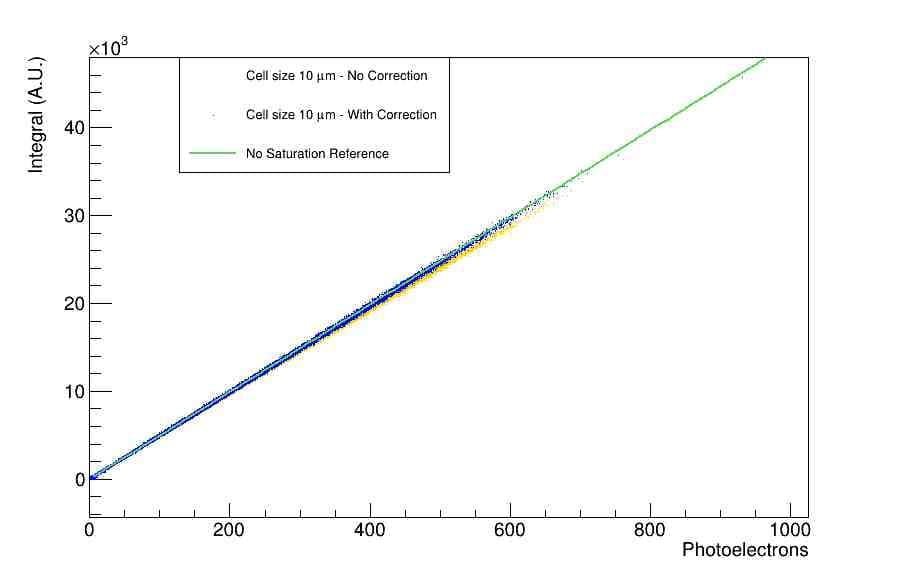
\includegraphics[width=.5\textwidth]{IMG/Cap5/SatCorr_40GeV_fib_cher}}\quad
	\subfloat[][Scintillation signals. Points are single SiPMs.]{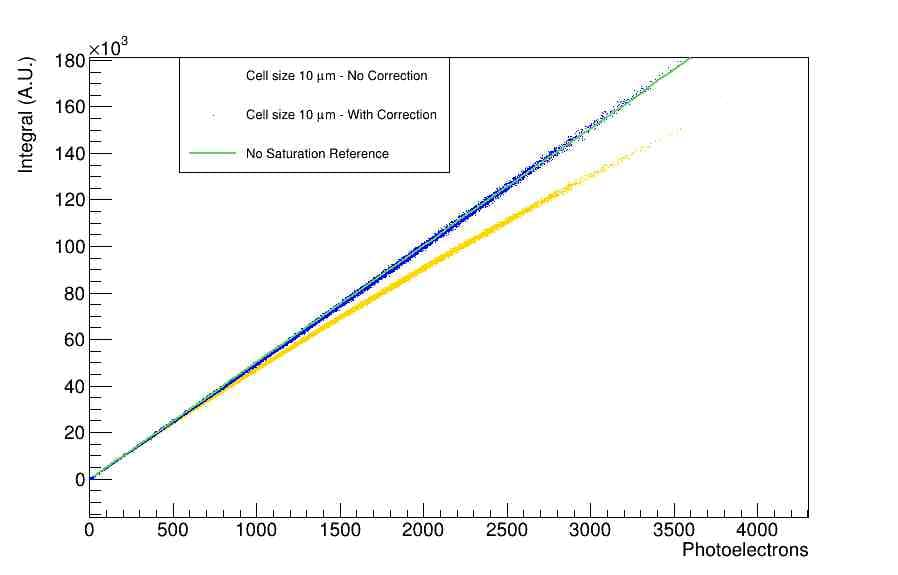
\includegraphics[width=.5\textwidth]{IMG/Cap5/SatCorr_40GeV_fib_scin}}\\
	\subfloat[][Cherenkov signals. Points are single events.]{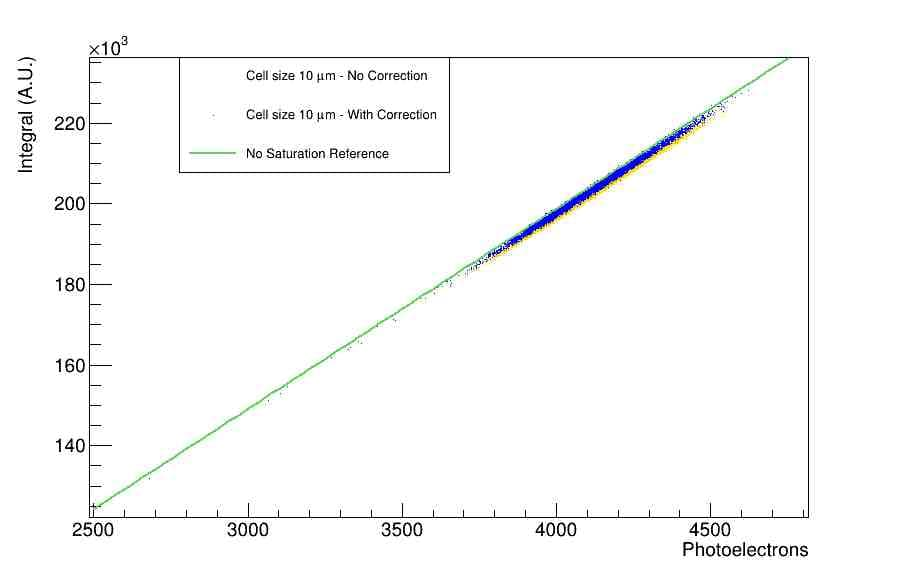
\includegraphics[width=.5\textwidth]{IMG/Cap5/SatCorr_40GeV_ev_cher}} \quad
	\subfloat[][Scintillation signals. Points are single events.]{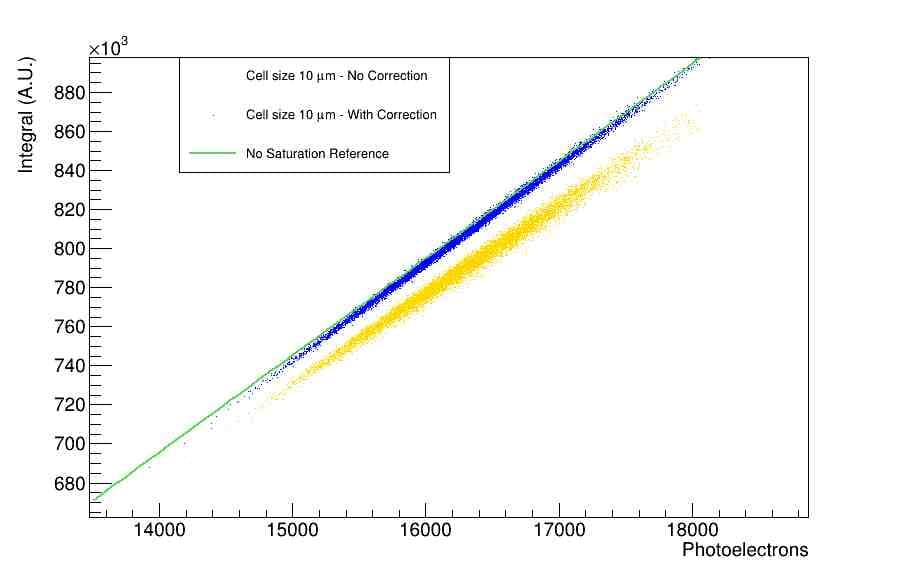
\includegraphics[width=.5\textwidth]{IMG/Cap5/SatCorr_40GeV_ev_scin}}
	\caption{Similar plots to figures \ref{fig:sat_fibres} and \ref{fig:sat_events}. Two series of data are presented to show the effectiveness of the analytical correction. The no saturation line shown in figure \ref{fig:NoSatLine} has been added as reference. }
	\label{fig:sat_corr}
\end{figure}

The discrepancy from the no saturation reference quantifies the effect of the occupancy when performing the energy reconstruction task. The percentage difference has been evaluated through the formula $\frac{E_{NoSat}-E}{E_{NoSat}}$, and the value obtained fill the histograms in figure \ref{fig:perc_sat}.\\
After applying the analytical correction a clear improvement is show in figures \ref{fig:sat_corr_perc}.\\

\begin{figure}
	\centering
	\subfloat[][Cherenkov signals.]{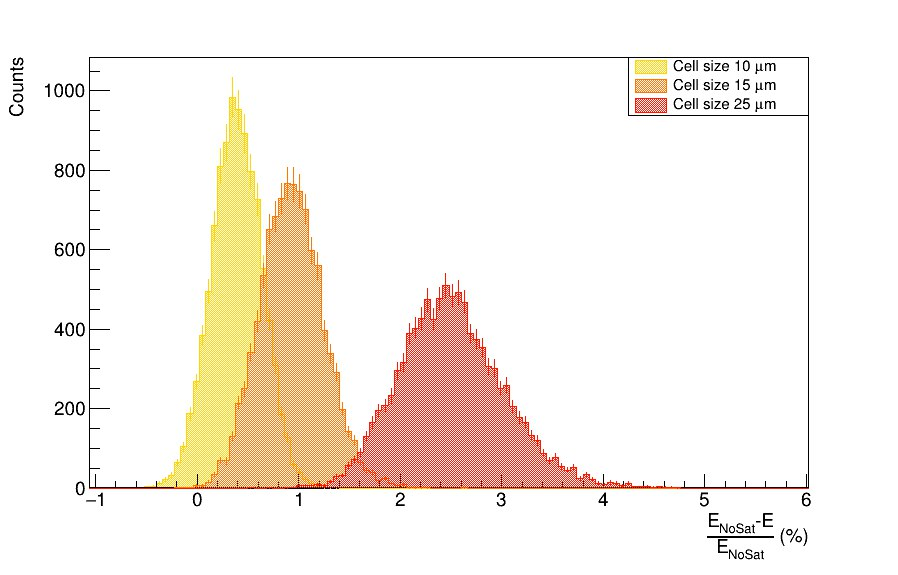
\includegraphics[width=.5\textwidth]{IMG/PercEnergy_40GeV_cher.jpg}} \quad
	\subfloat[][Scintillation signals.]{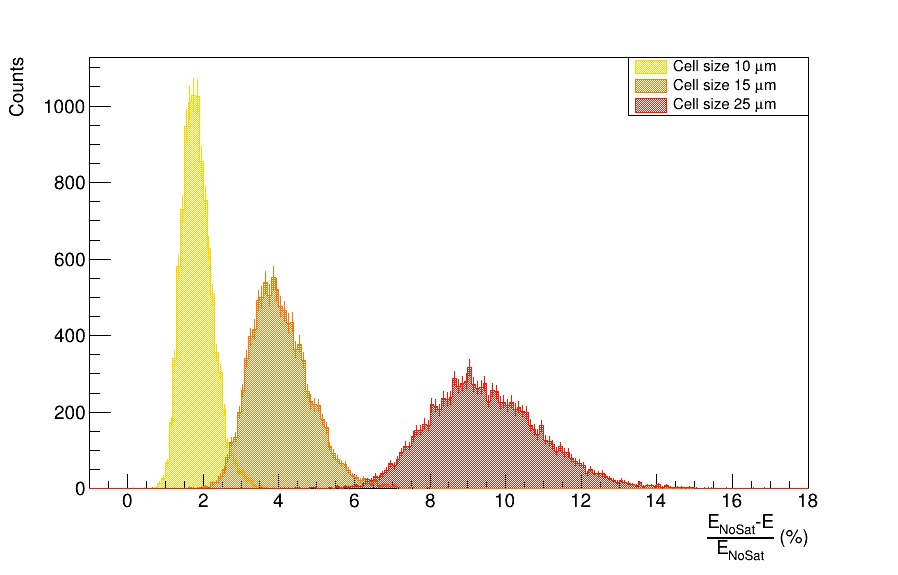
\includegraphics[width=.5\textwidth]{IMG/PercEnergy_40GeV_scin.jpg}}
	\caption{Percentage discrepancy distribution considering events with single 40GeV electrons. Different colors correspond to different cell size values.}
	\label{fig:sat_events}
\end{figure}

\begin{figure}
	\centering
	\subfloat[][Cherenkov signals.]{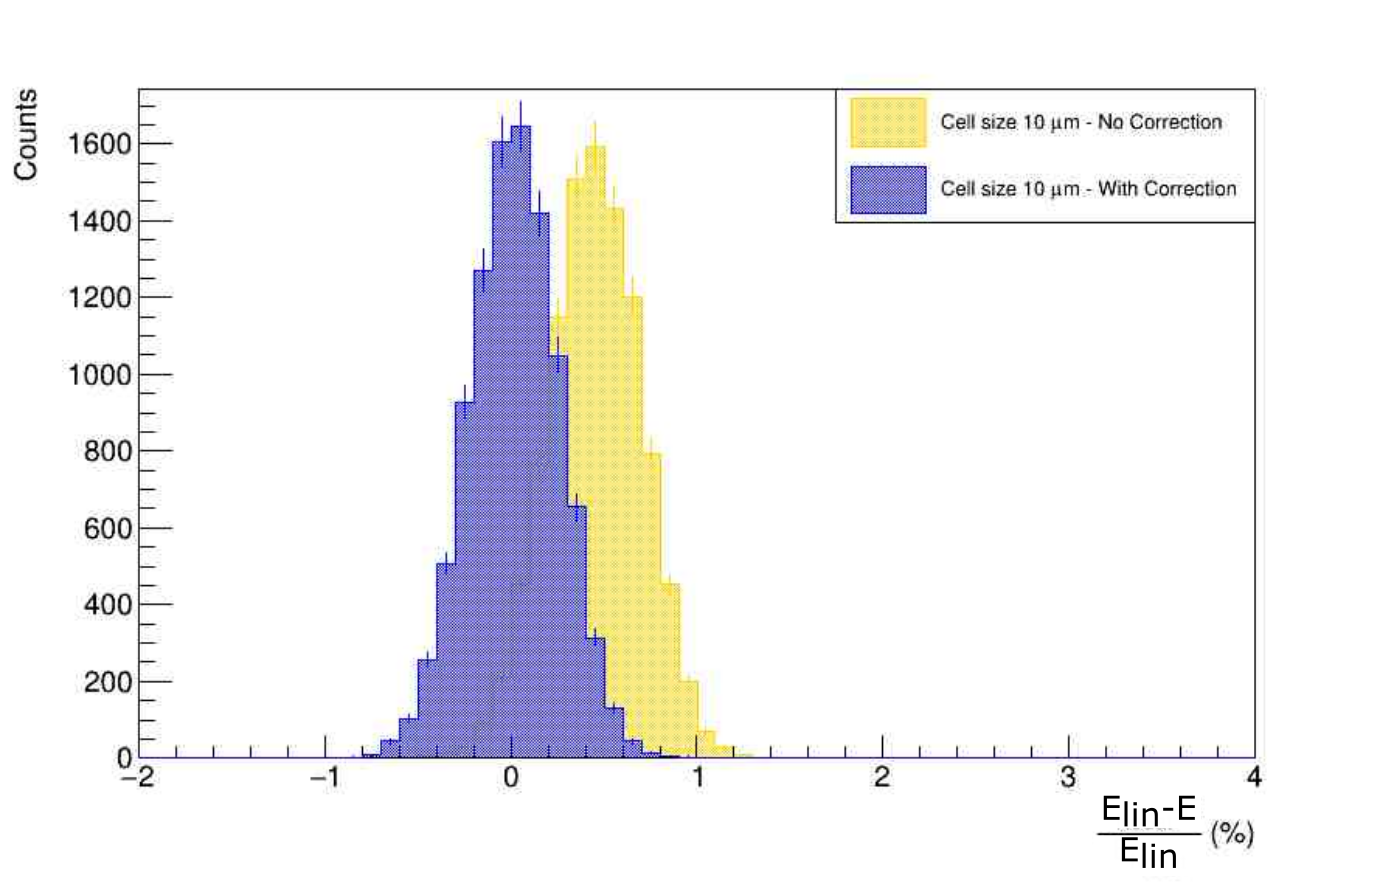
\includegraphics[width=.5\textwidth]{IMG/Cap5/PercEnergy_40GeV_corr_cher}} \quad
	\subfloat[][Scintillation signals.]{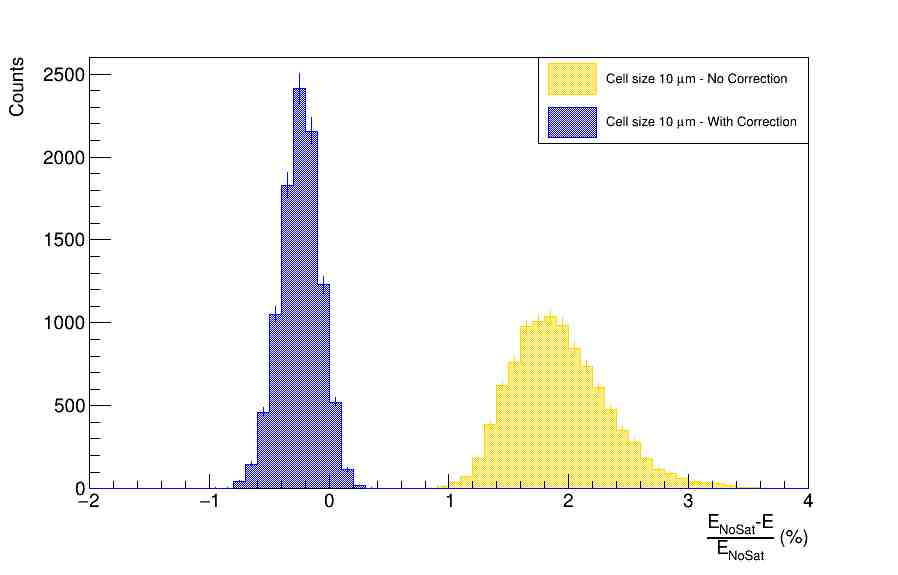
\includegraphics[width=.5\textwidth]{IMG/Cap5/PercEnergy_40GeV_corr_scin}}
	\caption{Percentage discrepancy distribution considering events with single 40GeV electrons to evaluate the effect of the analytical correction applied on data obtained with a cell size of $10\ \mu m$.}
		\label{fig:sat_corr_perc}
\end{figure}

This whole process has been performed simulating electrons with energies of $20,\ 40,\ 60,\ 80\ GeV$. Mean and standard deviation of the gaussian fit applied on the percentage discrepancy have been recorded and the obtained plots are shown in figure \ref{fig:sat_vs_E}.\\

\begin{figure}
	\centering
	\subfloat[][Cherenkov signals.]{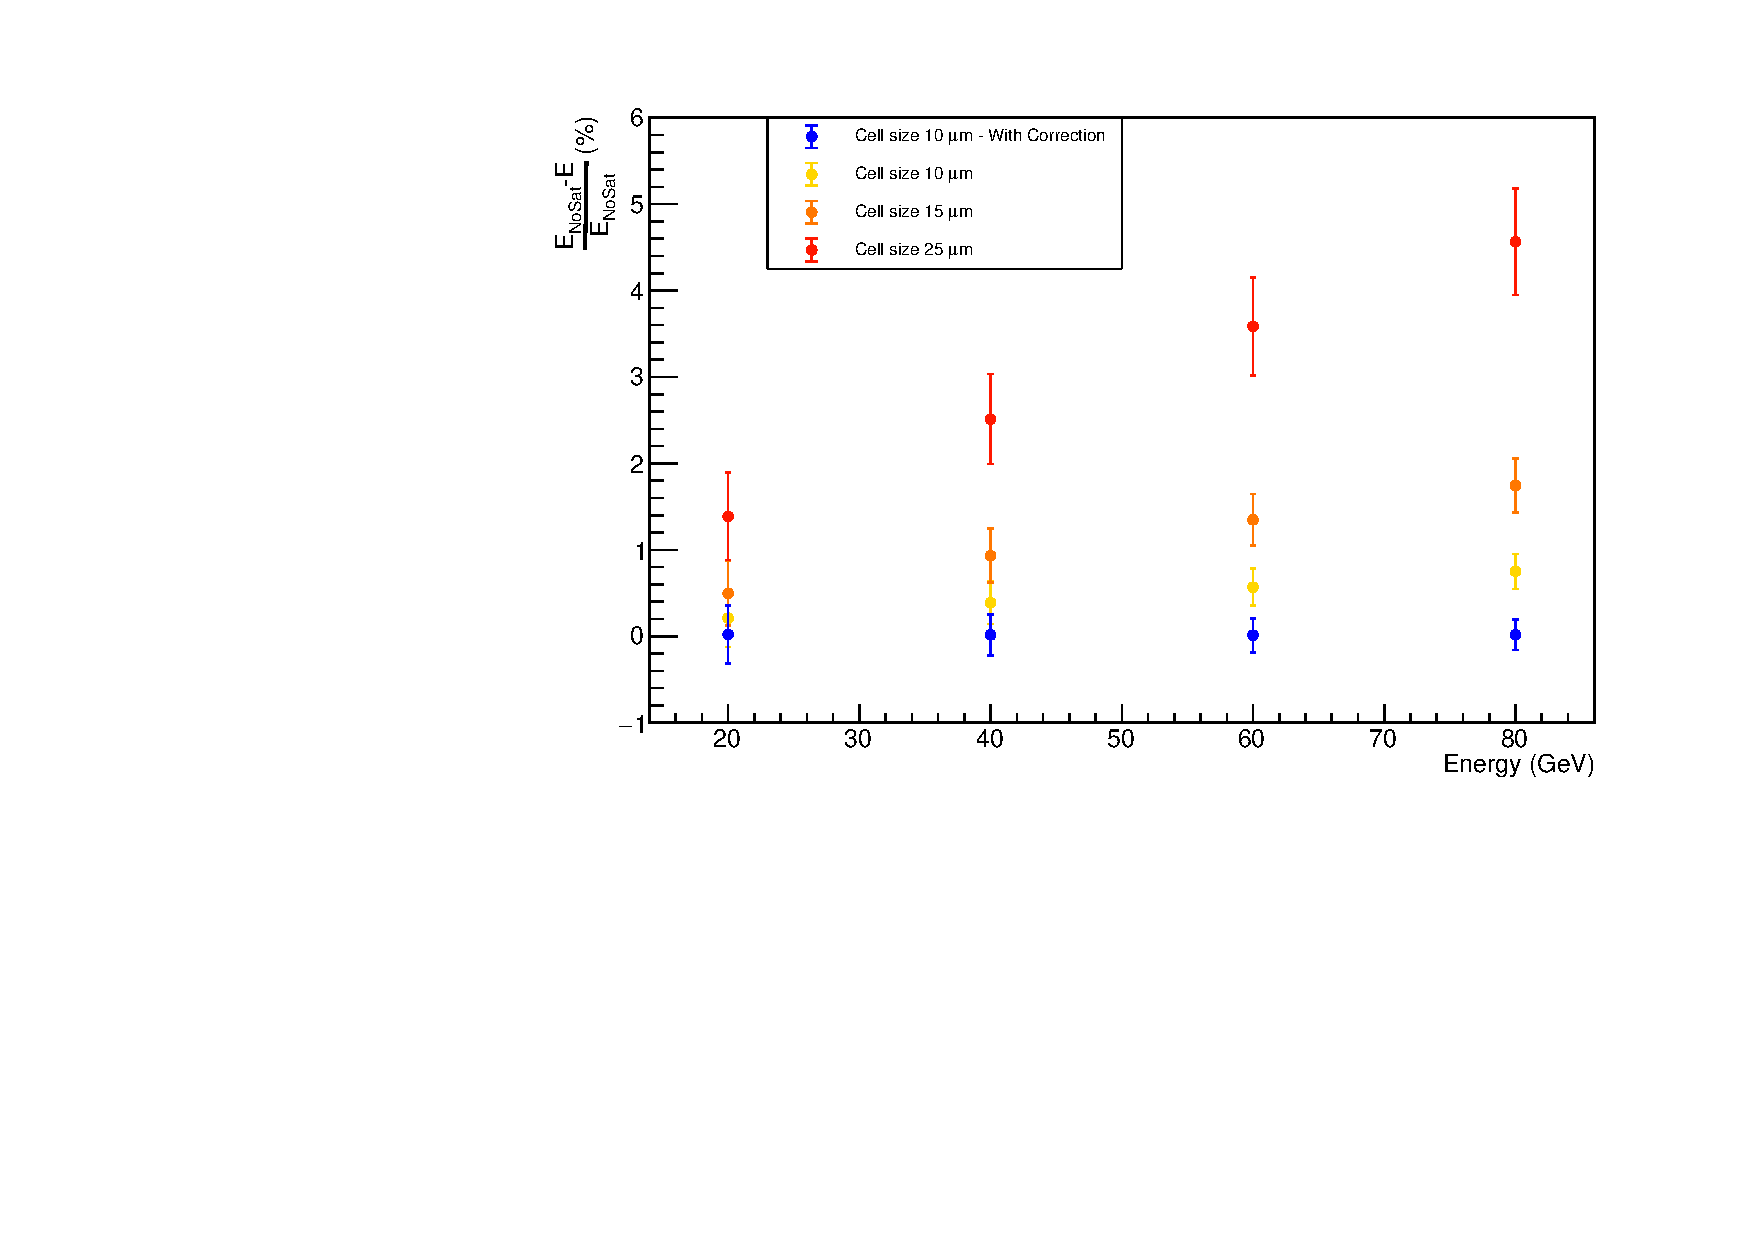
\includegraphics[width=.7\textwidth]{IMG/Cap5/PercEnergy_cher}} \\
	\subfloat[][Scintillation signals.]{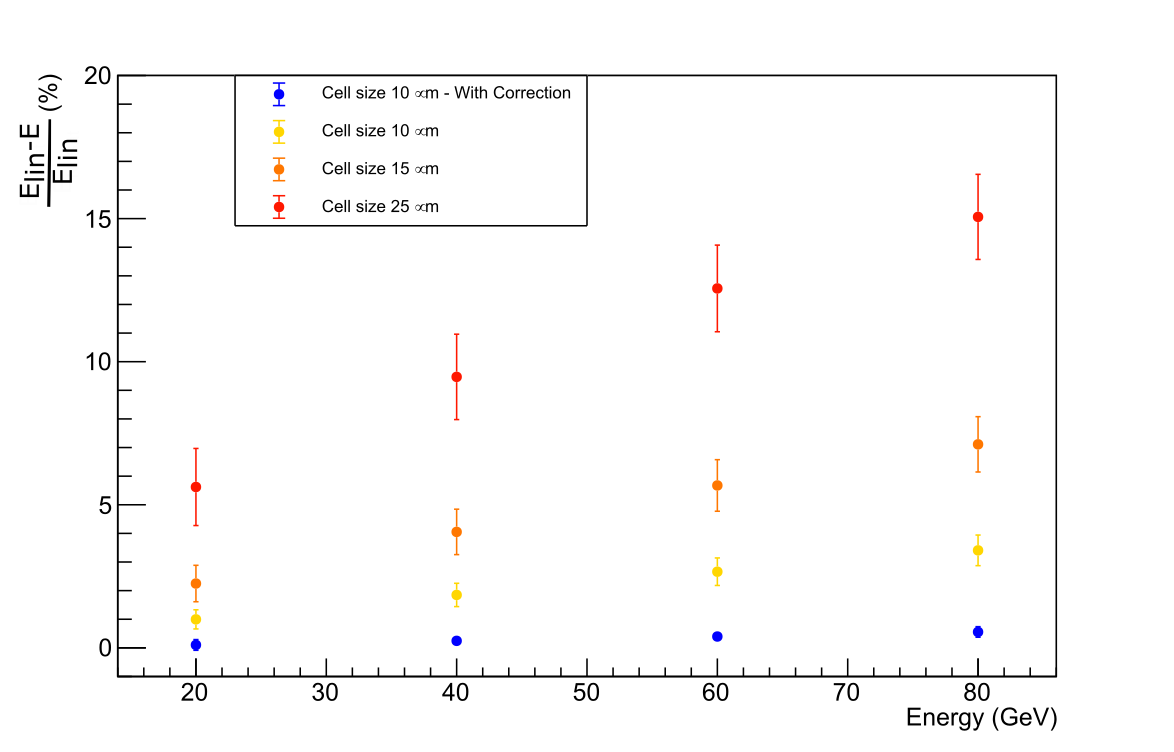
\includegraphics[width=.7\textwidth]{IMG/Cap5/PercEnergy_scin}}
	\caption{Percentage discrepancy behaviour with respect to the primary particle energy. Different cell sizes are compared also with data obtained performing the analytical correction.}
	\label{fig:sat_vs_E}
\end{figure}

\subsection{Energy resolution} \label{subsec:E_res}
The first step to study the energy resolution is to calibrate the full simulation.\\
Dual-readout calorimeters are typically calibrated at the electromagnetic scale. This is specially useful in a leptonic collider because, having easily access to electrons and positrons, the calorimeter can be calibrated precisely during all the life of the experiment.\\

The calibration has been performed on $40\ GeV$ electrons applying the one-suppression already introduce in paragraph \ref{subsec:Sim_SiPM}. $10000$ events with single $40\ GeV$ electrons have been fired from the interaction point obtaining the charge integral distributions for scintillation and Cherenkov signals.% shown in figure \ref{fig:int_dist}.
The calibration constants obtained to transform these data in energy distributions centered around $40\ GeV$ are: $k_S = 4.998 \times 10^{-5}$ and $k_C = 2.023 \times 10^{-4}$.\\
Two analogue calibration constants have been obtained starting from the number of photoelectrons distribution with values of:  $k_{pe,S} = 2.48 \times 10^{-3}$ and $k_{pe,C} = 1.00 \times 10^{-2}$.\\

%\begin{figure}
%	\centering
%	\subfloat[][Cherenkov signals.]{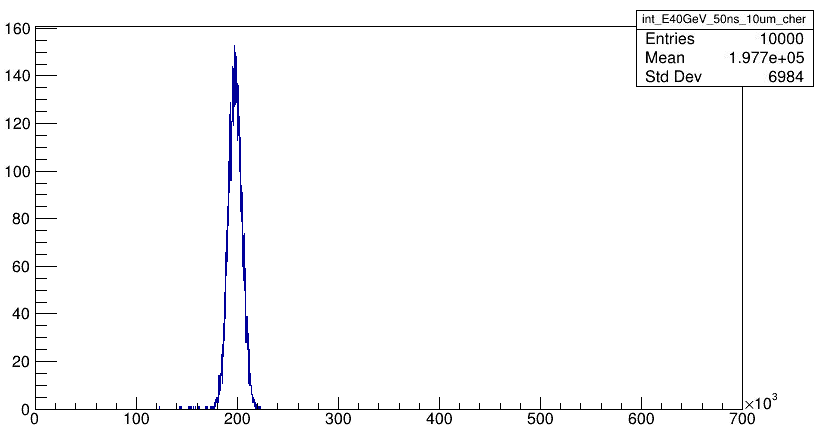
\includegraphics[width=.7\textwidth]{IMG/Intdist_40GeV_cher_cal}} \\
%	\subfloat[][Scintillation signals.]{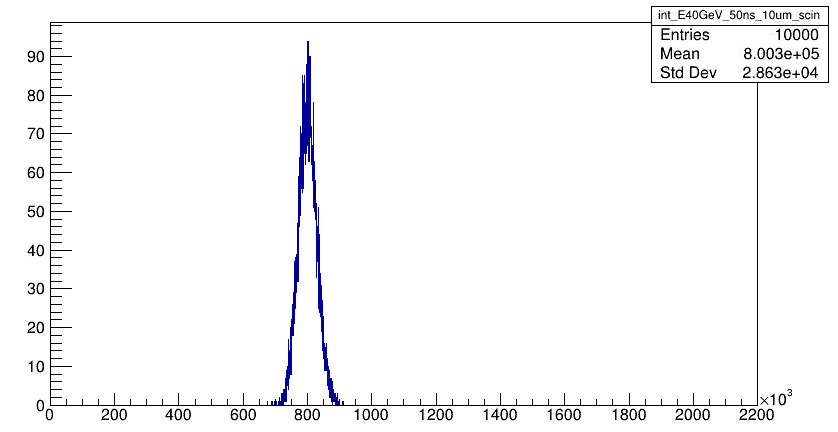
\includegraphics[width=.7\textwidth]{IMG/Intdist_40GeV_scin_cal}}
%	\caption{Integral distrib.}
%	\label{fig:int_dist}
%\end{figure}

Starting from these calibration constant, the energy distributions can be obtained from the number of p.e. (pre SiPM digitization simulation) or from the charge integral (post SiPM digitization simulation). The two types of distribution are compared in figure \ref{fig:cfr_e_dist}.\\
As expected, the energy distributions obtained from the charge integrals are wider due to the introduction of the electronic noise. However, the effect is extremely minimal considering the fact that in each event hundreds of SiPMs are active.\\
%and the white noise has mean zero.

\begin{figure}
	\centering
	\subfloat[][Cherenkov signals.]{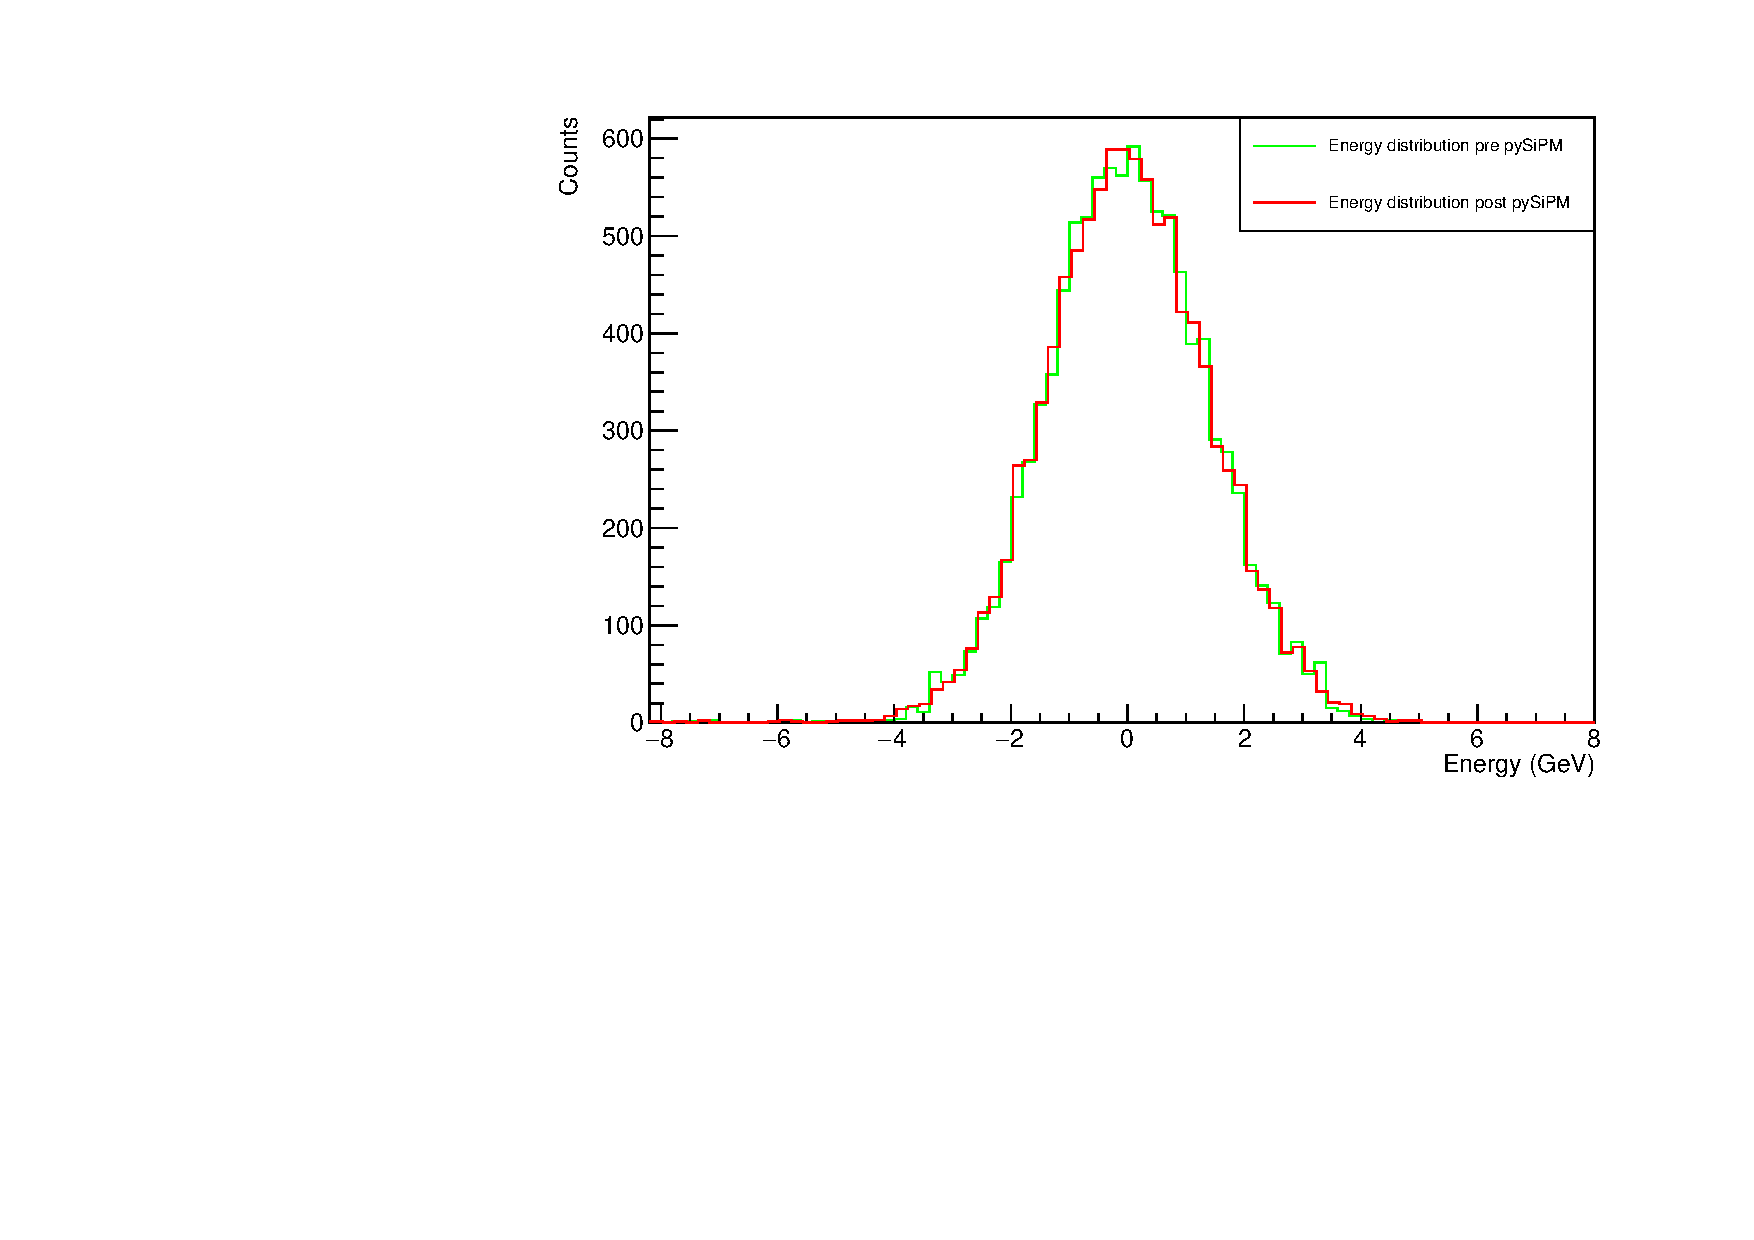
\includegraphics[width=.7\textwidth]{IMG/Cap5/E_hist_cfr_cher}} \\
	\subfloat[][Scintillation signals.]{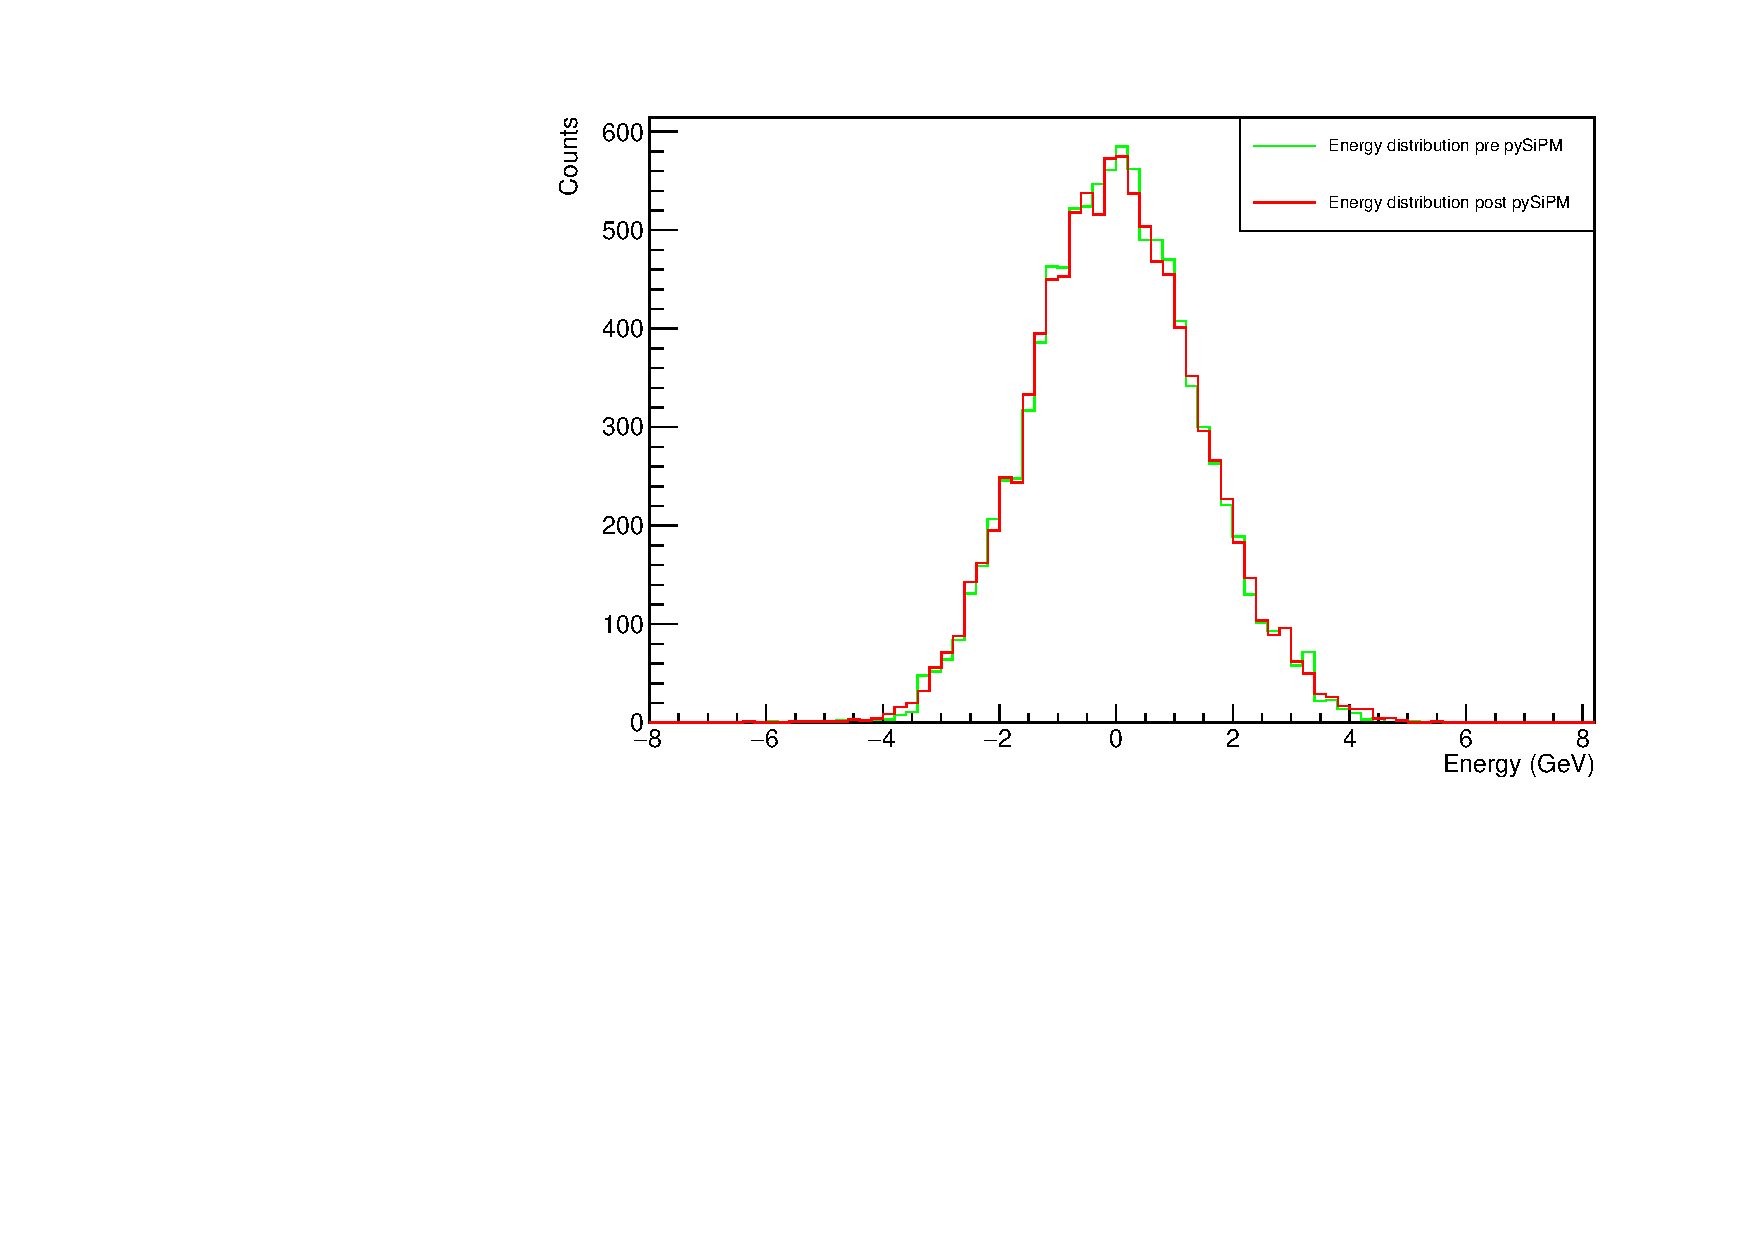
\includegraphics[width=.7\textwidth]{IMG/Cap5/E_hist_cfr_scin}}
	\caption{Charge integral distributions generated with data from GEANT4 (\textit{pre pySiPM}) or from the full simulation (\textit{post pySiPM}). The histograms are shifted by their mean values to show the minimal difference in the distributions spread.}
	\label{fig:cfr_e_dist}
\end{figure}

The energy distributions have been fitted with a Gaussian function to obtain mean, standard deviation e respective errors. Doing this with different primary electron energies the energy resolution can be studied. Mean and standard deviation are listed in tables \ref{tab:e_res_int} \ref{tab:e_res_pe}.\\
Then, fitting the $\sigma/E$ values obtained from photoelectron number in the energy range $5-80\ GeV$, can be seen there is a good agreement with the function:
\begin{equation}\label{eq:resolution}
	%\frac{\sigma}{E} = \frac{A_1}{\sqrt{E}} + B_1 \qquad \text{or} \qquad \frac{\sigma}{E} = \frac{A_2}{\sqrt{E}} \oplus B_2
	\frac{\sigma}{E} = \frac{A}{\sqrt{E}} \oplus B.
\end{equation} 
On the other hand, adding the SiPM digitization, an uncorrelated electrical error has to be added in quadrature, therefore the fit function became:
\begin{equation}\label{eq:resolution}
	%\frac{\sigma}{E} = \frac{A_1}{\sqrt{E}} + B_1 \qquad \text{or} \qquad \frac{\sigma}{E} = \frac{A_2}{\sqrt{E}} \oplus B_2
	\frac{\sigma}{E} = \frac{A}{\sqrt{E}} \oplus B \oplus \frac{C}{E},
\end{equation} 
where the parameters $A$ and $B$, that in first approximation should not be affected by the digitization, have been fixed as the one obtained before. The plots are shown in figure \ref{fig:sigma_su_e}, with the fit parameters listed in table \ref{tab:res_regular_sum}. They also show that the loss of resolution with the introduction of the SiPM digitization software is minimal.\\
% and \ref{tab:res_quadratic_sum}

\begin{table}
	\centering
	\begin{tabular}{lccc}
		\toprule
		& True E (GeV) & Mean E (GeV) & Standard Deviation (GeV) \\
		\midrule
		\textbf{Scintillation} &	$5$ 	& $4.91$ & $0.42$ \\
		& $20$ 	& $19.90$ & $0.92$ \\
		& $40$ 	& $40.00$ & $1.42$ \\
		& $60$ 	& $60.65$ & $1.83$ \\
		& $80$ 	& $81.18$ & $2.22$ \\
		\midrule
		\textbf{Cherenkov} & $5$ 	& $4.80$ & $0.45$ \\
		& $20$ 	& $19.88$ & $0.91$ \\
		& $40$ 	& $40.00$ & $1.36$ \\
		& $60$ 	& $60.63$ & $1.66$ \\
		& $80$ 	& $81.12$ & $1.92$ \\
		\bottomrule		
	\end{tabular}
	\caption{Mean and standard deviation obtained by fitting with Gaussian function the energy distributions. The data are obtained with results from the full simulation.}
	\label{tab:e_res_int}
\end{table}

\begin{table}
	\centering
	\begin{tabular}{lccc}
		\toprule
		& True E (GeV) & Mean E (GeV) & Standard Deviation (GeV) \\
		\midrule
		\textbf{Scintillation} &	$5$ 	& $4.91$ & $0.41$ \\
		& $20$ 	& $19.90$ & $0.92$ \\
		& $40$ 	& $40.00$ & $1.39$ \\
		& $60$ 	& $60.65$ & $1.78$ \\
		& $80$ 	& $81.18$ & $2.16$ \\
		\midrule
		\textbf{Cherenkov} & $5$ 	& $4.77$ & $4.48$ \\
		& $20$ 	& $19.76$ & $0.92$ \\
		& $40$ 	& $40.00$ & $1.36$ \\
		& $60$ 	& $60.40$ & $1.66$ \\
		& $80$ 	& $81.86$ & $1.91$ \\
		\bottomrule
	\end{tabular}
	\caption{Mean and standard deviation obtained by fitting with Gaussian function the energy distributions. The data are obtained with results from DR calorimeter simulation applying the calibration from the photoelectrons number.}
	\label{tab:e_res_pe}
\end{table}

\begin{figure}
	\centering
	\subfloat[][$C$ signals.]{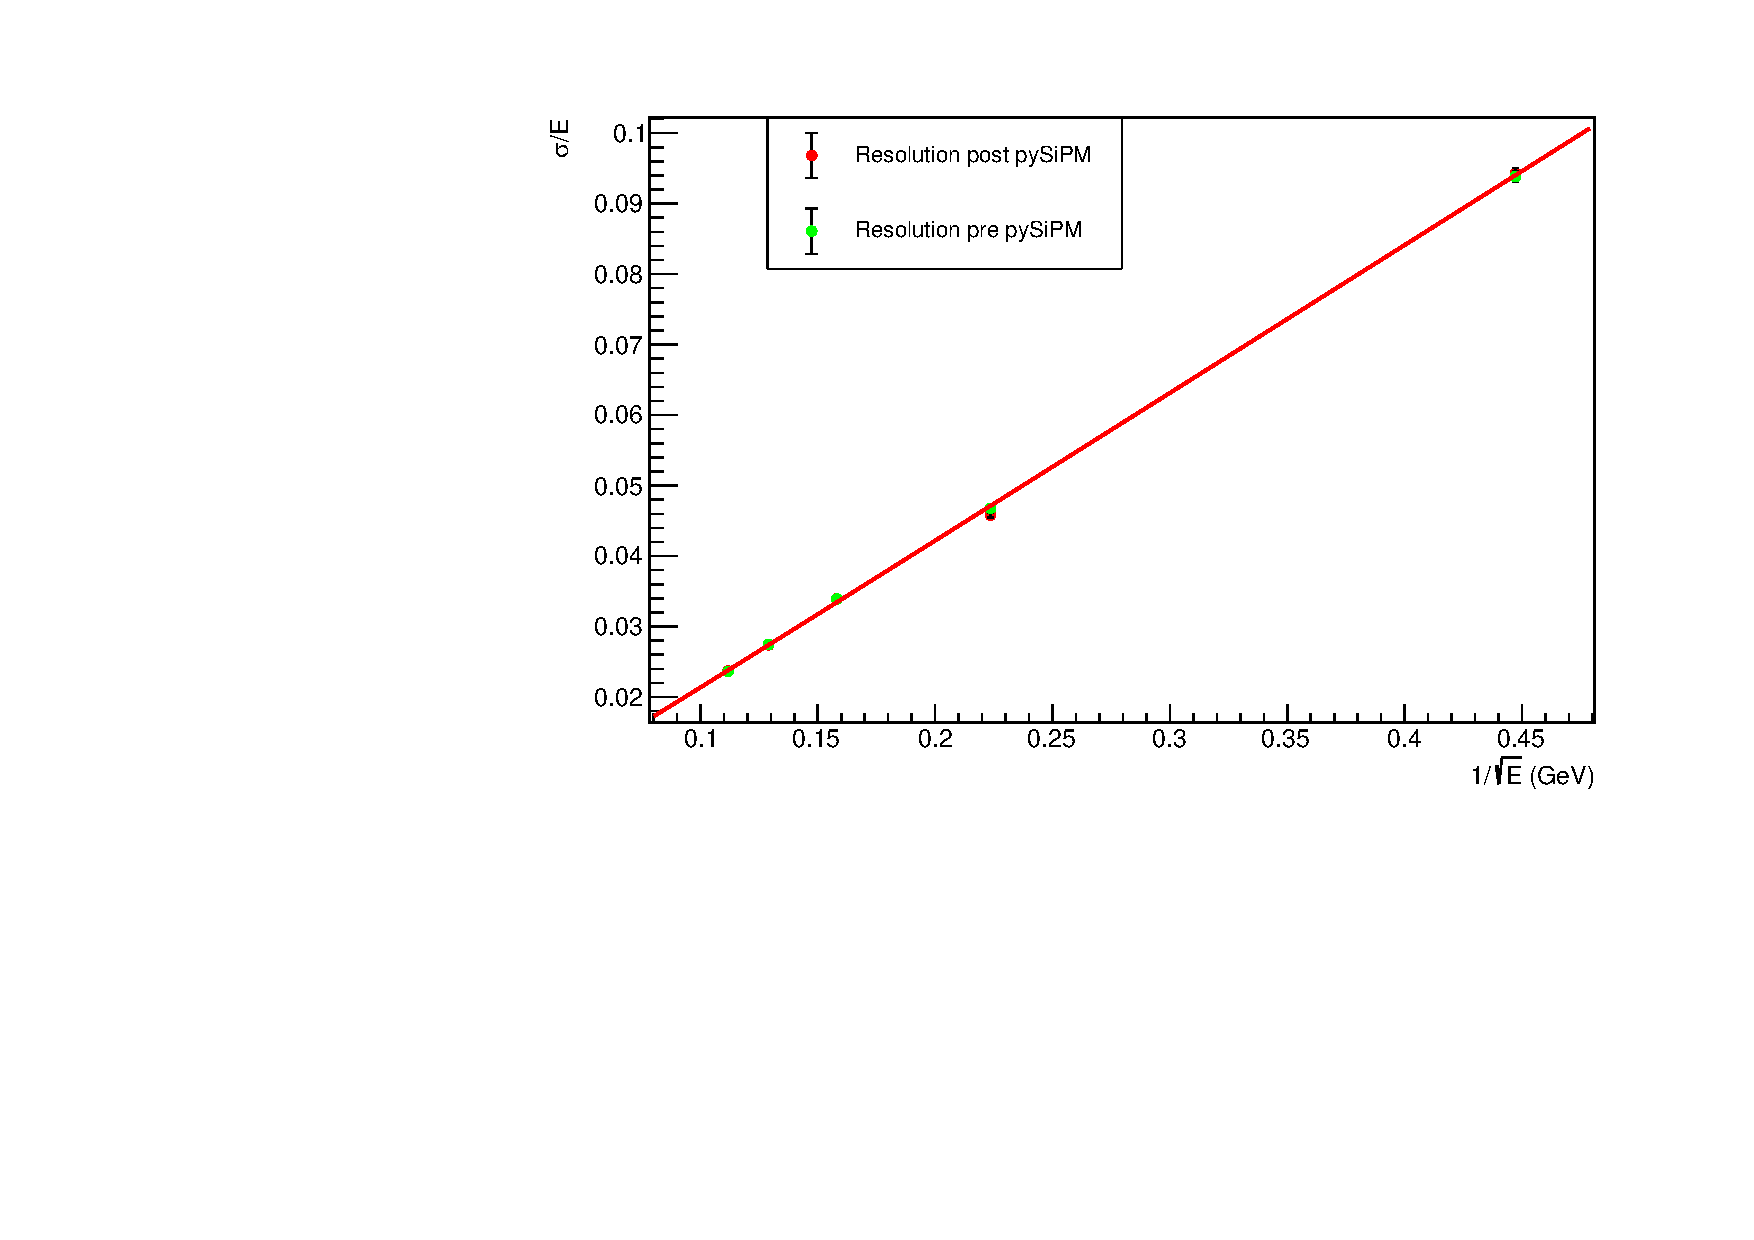
\includegraphics[width=.8\textwidth]{IMG/Cap5/Res_cher.pdf}} \\
	\subfloat[][$S$ signals.]{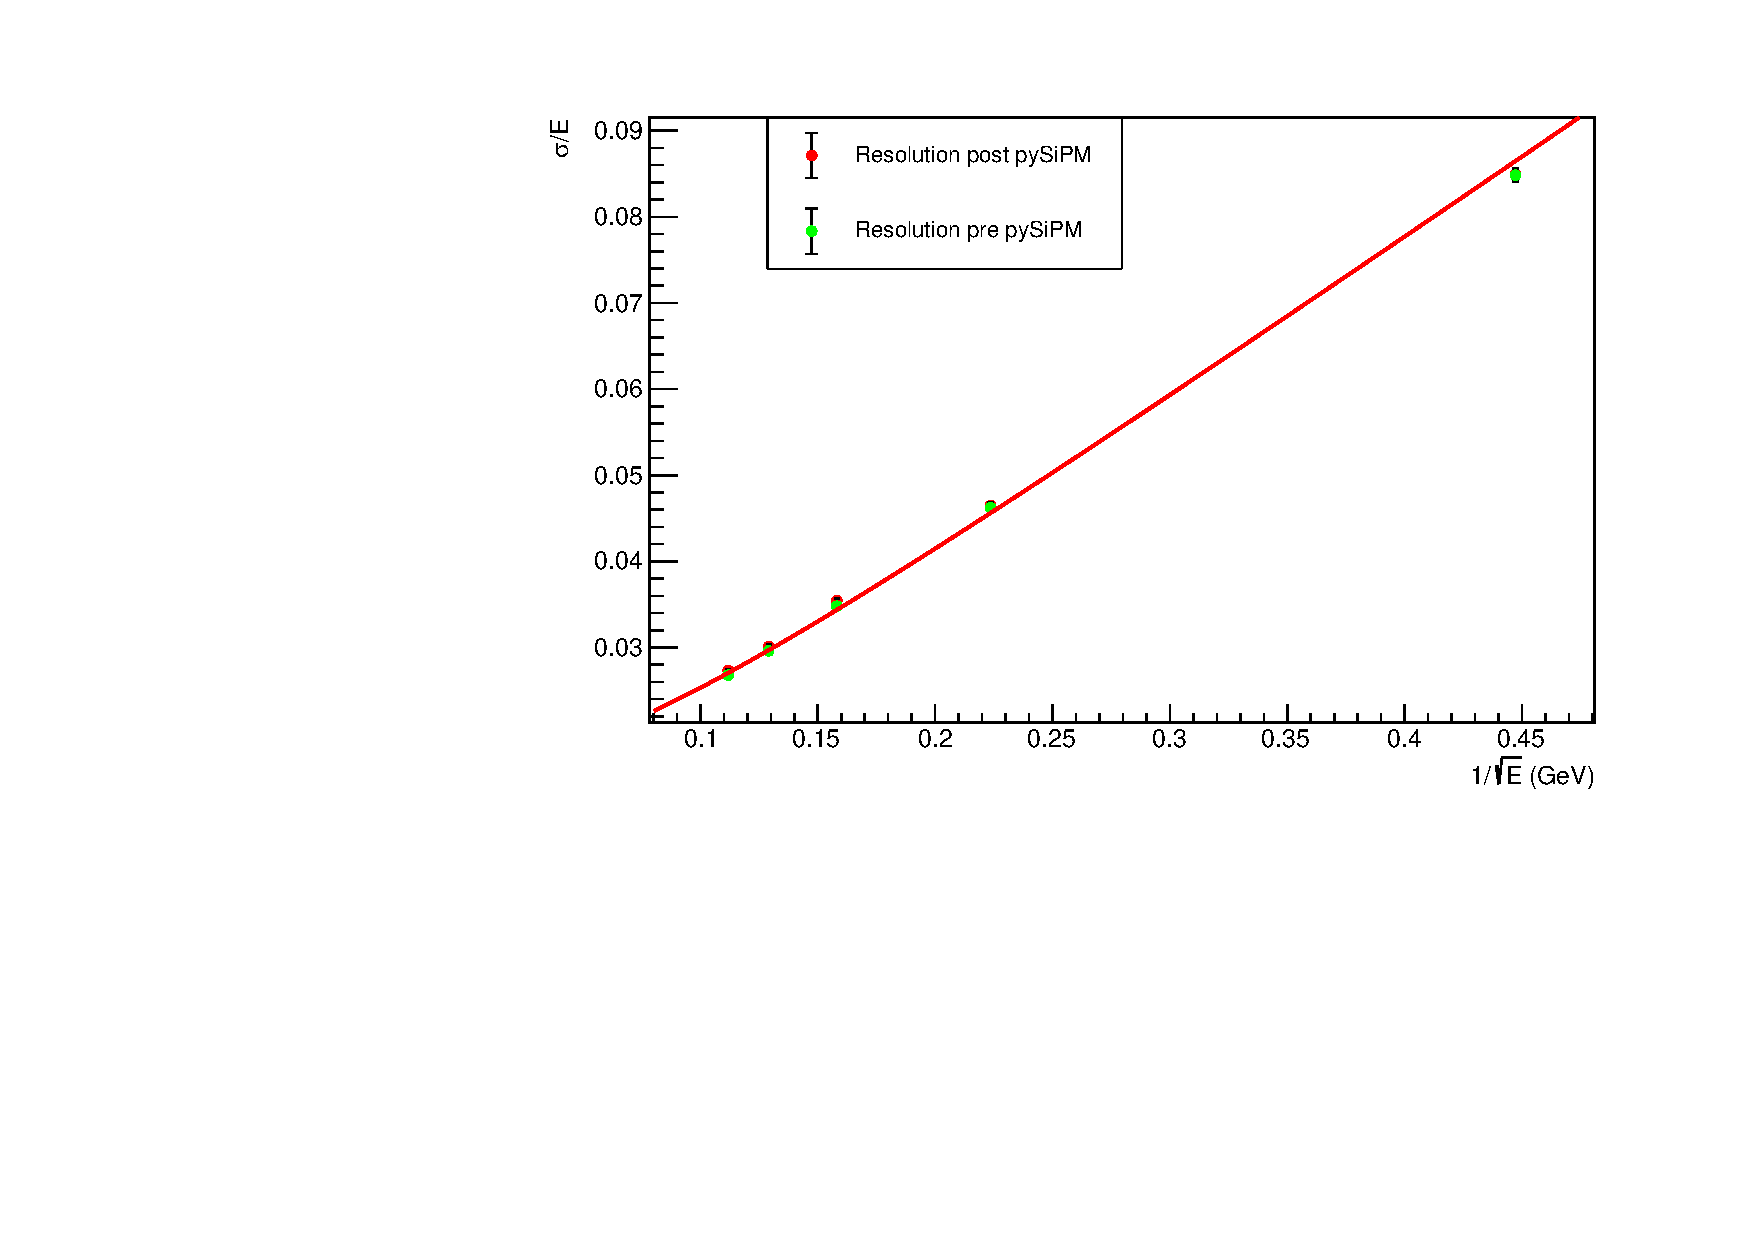
\includegraphics[width=.8\textwidth]{IMG/Cap5/Res_scin.pdf}}
	\caption{Calorimeter resolution plot where the data have been fitted with the formula \ref{eq:resolution}.}
	\label{fig:sigma_su_e}
\end{figure}

\begin{table}
	\centering
	\begin{tabular}{lcc}
		\toprule
		& \textbf{Scintillation} & \textbf{Cherenkov} \\
		\midrule
		\textbf{pre pySiPM} &	$\frac{\sigma}{E} = \frac{18.97\%}{\sqrt{E}} \oplus 1.677\%$ 	& $\frac{\sigma}{E} = \frac{21.01\%}{\sqrt{E}} \oplus 0.386\%$ \\
		%\textbf{post pySiPM} & $\frac{\sigma}{E} = \frac{18.97\%}{\sqrt{E}} \oplus 1.677\% \oplus \frac{1.975\cdot 10^{-6}\%}{E}$ 	& $\frac{\sigma}{E} = \frac{21.01\%}{\sqrt{E}} \oplus 0.386\% \oplus \frac{4.226\cdot 10^{-4}\%}{E}$ \\
		\textbf{post pySiPM} & \dots $\oplus \frac{1.975\cdot 10^{-6}\%}{E}$ 	& \dots $\oplus \frac{4.226\cdot 10^{-4}\%}{E}$ \\
		\bottomrule
	\end{tabular}
	\caption{Fit results on the energy resolution using the functional form \ref{eq:resolution}.}
	\label{tab:res_regular_sum}
\end{table}

%\begin{table}
%	\centering
%	\begin{tabular}{lcc}
%		\toprule
%		& \textbf{Scintillation} & \textbf{Cherenkov} \\
%		\midrule
%		\textbf{pre pySiPM} &	$\frac{19.78\%}{\sqrt{E}}\oplus1.55\%$ 	& $\frac{21.21\%}{\sqrt{E}}\oplus0.07\%$ \\
%		\textbf{post pySiPM} & $\frac{20.14\%}{\sqrt{E}}\oplus1.62\%$ 	& $\frac{21.04\%}{\sqrt{E}}\oplus0.98\%$ \\
%		\bottomrule
%	\end{tabular}
%	\caption{Fit results on the energy resolution using the functional form \ref{eq:resolution} on the right.}
%	\label{tab:res_quadratic_sum}
%\end{table}